%% This is an example first chapter.  You should put chapter/appendix that you
%% write into a separate file, and add a line \include{yourfilename} to
%% main.tex, where `yourfilename.tex' is the name of the chapter/appendix file.
%% You can process specific files by typing their names in at the 
%% \files=
%% prompt when you run the file main.tex through LaTeX.
\chapter{Event Reconstruction}

\section{Track reconstruction}

The goal of the track reconstruction is to estimate the position and momentum parameters of charged particles from the reconstructed hits in the inner tracking detector. Reconstructing tracks at the LHC nominal instantaneous luminosities is computationally challenging due to high occupancy environment. About $1000$ charged particles transverse the inner tracking detectors. Charged particles from prior or later bunch crossings can also be present due to finite detector time resolution.  The track reconstruction starts by clustering of zero-suppressed signals in the pixel and strip detectors into hits with an estimate of the cluster positions and the corresponding uncertainties. The CMS track reconstruction algorithm is referred to as combinational track finder (CTF)~\cite{Adam:934067,Chatrchyan:2014fea}. The CTF is an adaptation of the combinatorial Kalman filter~\cite{BILLOIR1989390,BILLOIR1990219,MANKEL1997169}, which is an extension of the Kalman filter~\cite{FRUHWIRTH1987444} to combine the pattern recognition and track fitting in the same framework. 

The CTF is performed six times to determine the collection of the tracks in an event. The aim of this iterative tracking is to first find the tracks that are easiest to find (high $p_{T}$ and near the interaction region) with subsequent iterations searching for the more challenging tracks (low $p_{T}$ and displaced from the interaction region). Hits associated with tracks are removed after each iteration thereby reducing the computational complexity. Each iteration has four steps:

\begin{description}
\item[$\bullet$ Seed generation:]  Initial track candidates are found using only two or three hits in the inner part of the tracker. One has to note that the seeds are not constructed from the outermost regions of the tracker where the track density is small. The high granularity of the pixel detector ensures that the channel occupancy is lower than the channel occupancy of the outer strip layers. In addition, significant fraction of charged pions undergo inelastic interaction in the track detectors while many electrons loose significant energy due to bremsstrahlung radiation as they transverse the tracker. There are five parameters needed to define the helical trajectory of the charged particles in the approximately uniform magnetic field. Two or three hits along with constraining the origin of the charged particle near the beam spot (the three dimensional profile of the luminous region of the collisions) is sufficient to extract these parameters.
\item[$\bullet$ Track finding:]  The Kalman filter algorithm is used to provide a coarse estimate of the track parameters starting from the seeds.  track candidate is built by adding hits from successive detector layers. A fast analytical propagator is used to find the hit layers. The track parameters are updated each time a new hit is found.
\item[$\bullet$ Track fitting:] The full information needed for the trajectory is only available once all the hits of the trajectory are identified. Therefore, the trajectory is once again re-fitted using a Kalman filter and smoother. A fourth-order Runge-Kutta method is used to extrapolate the trajectory between the successive hits. Material and inhomogeneous magnetic field effects are included.
\item[$\bullet$ Track selection:] Quality requirements are applied to reject fake tracks not originating from a charged particle. 
\end{description}

The track reconstruction is effectively fully efficient for isolated muons with $2.5\%$ resolution in $p_{T}$ for $p_{T}$ of about $100~\GeV$~\cite{Chatrchyan:2014fea}. The longitudinal (with respect to the $z$ axis) and transverse impact parameter resolutions are $30$ $\mu$m and $10$ $\mu$m respectively. The efficiency for charged particles of $p_{T}$ greater than $0.9~\GeV$ in simulated $t\bar{t}$ events is $94\%$ ($85\%$) in the pseudorapidity region of $|\eta|<0.9$ ($0.9<|\eta|<2.4$). The main cause of the inefficiency is due to the hadrons undergoing nuclear interactions in the tracker material.   

\section{Primary vertex reconstruction}

The goal of primary vertex reconstruction is to measure the position of each proton-proton interaction vertex in each event. The vertex reconstruction starts from the collection of the reconstructed tracks consistent with being produced near the beam spot. Additional quality requirements on the number of tracker layers associated to the track and the quality of the CTF fit are required. There is no requirement on the $p_{T}$ of the tracks ensuring high vertex reconstruction efficiency.

A clustering algorithm based on the $z$ coordinates of closest approach of the tracks to the beam spot is used to resolve the vertices. The tradeoff is to be able to resolve the nearby vertices against the accidental splitting of a single vertex into more than one cluster of tracks.  A deterministic annealing (DA) algorithm~\cite{726788} is used for the clustering where the most probable vertex positions are found through a minimization of "free energy" $F$ at "temperature" $T$~\cite{Chatrchyan:2014fea}, 
\begin{equation} \label{eq:minimize}
F = -T \sum_{i}^{N_{T}} \ln \sum_{j}^{N_{V}} p_{ij} \rho_{j} \exp  \left[-\frac{1}{T}\frac{(z_{i}^{T}-z_{j}^{V})^2}{{\sigma_{i}^{z}}^2} \right],
\end{equation}
where $z_{i}^{T}$ and $\sigma_{i}^{z}$ are the $z$ coordinates of the points of the closest approach of the tracks to the $z$ and the corresponding uncertainties, $z_{j}^{V}$ are the vertex positions with vertex weights $\rho_{j}$, and $p_{ij}$ is the probability of assigning the track $i$ to the vertex $j$. The assignment of the probabilities is such that at very low temperatures every track is compatible with a single vertex while at very high temperatures all the tracks become compatible with a single vertex. The algorithm starts at a high temperature that gradually decreases ($F$ is minimized at each step) until a pre-defined minimum temperature is reached. Thereafter the temperature is further decreased to $T=1$ for the final assignment without further splitting. 

\begin{figure}[h]
\centering
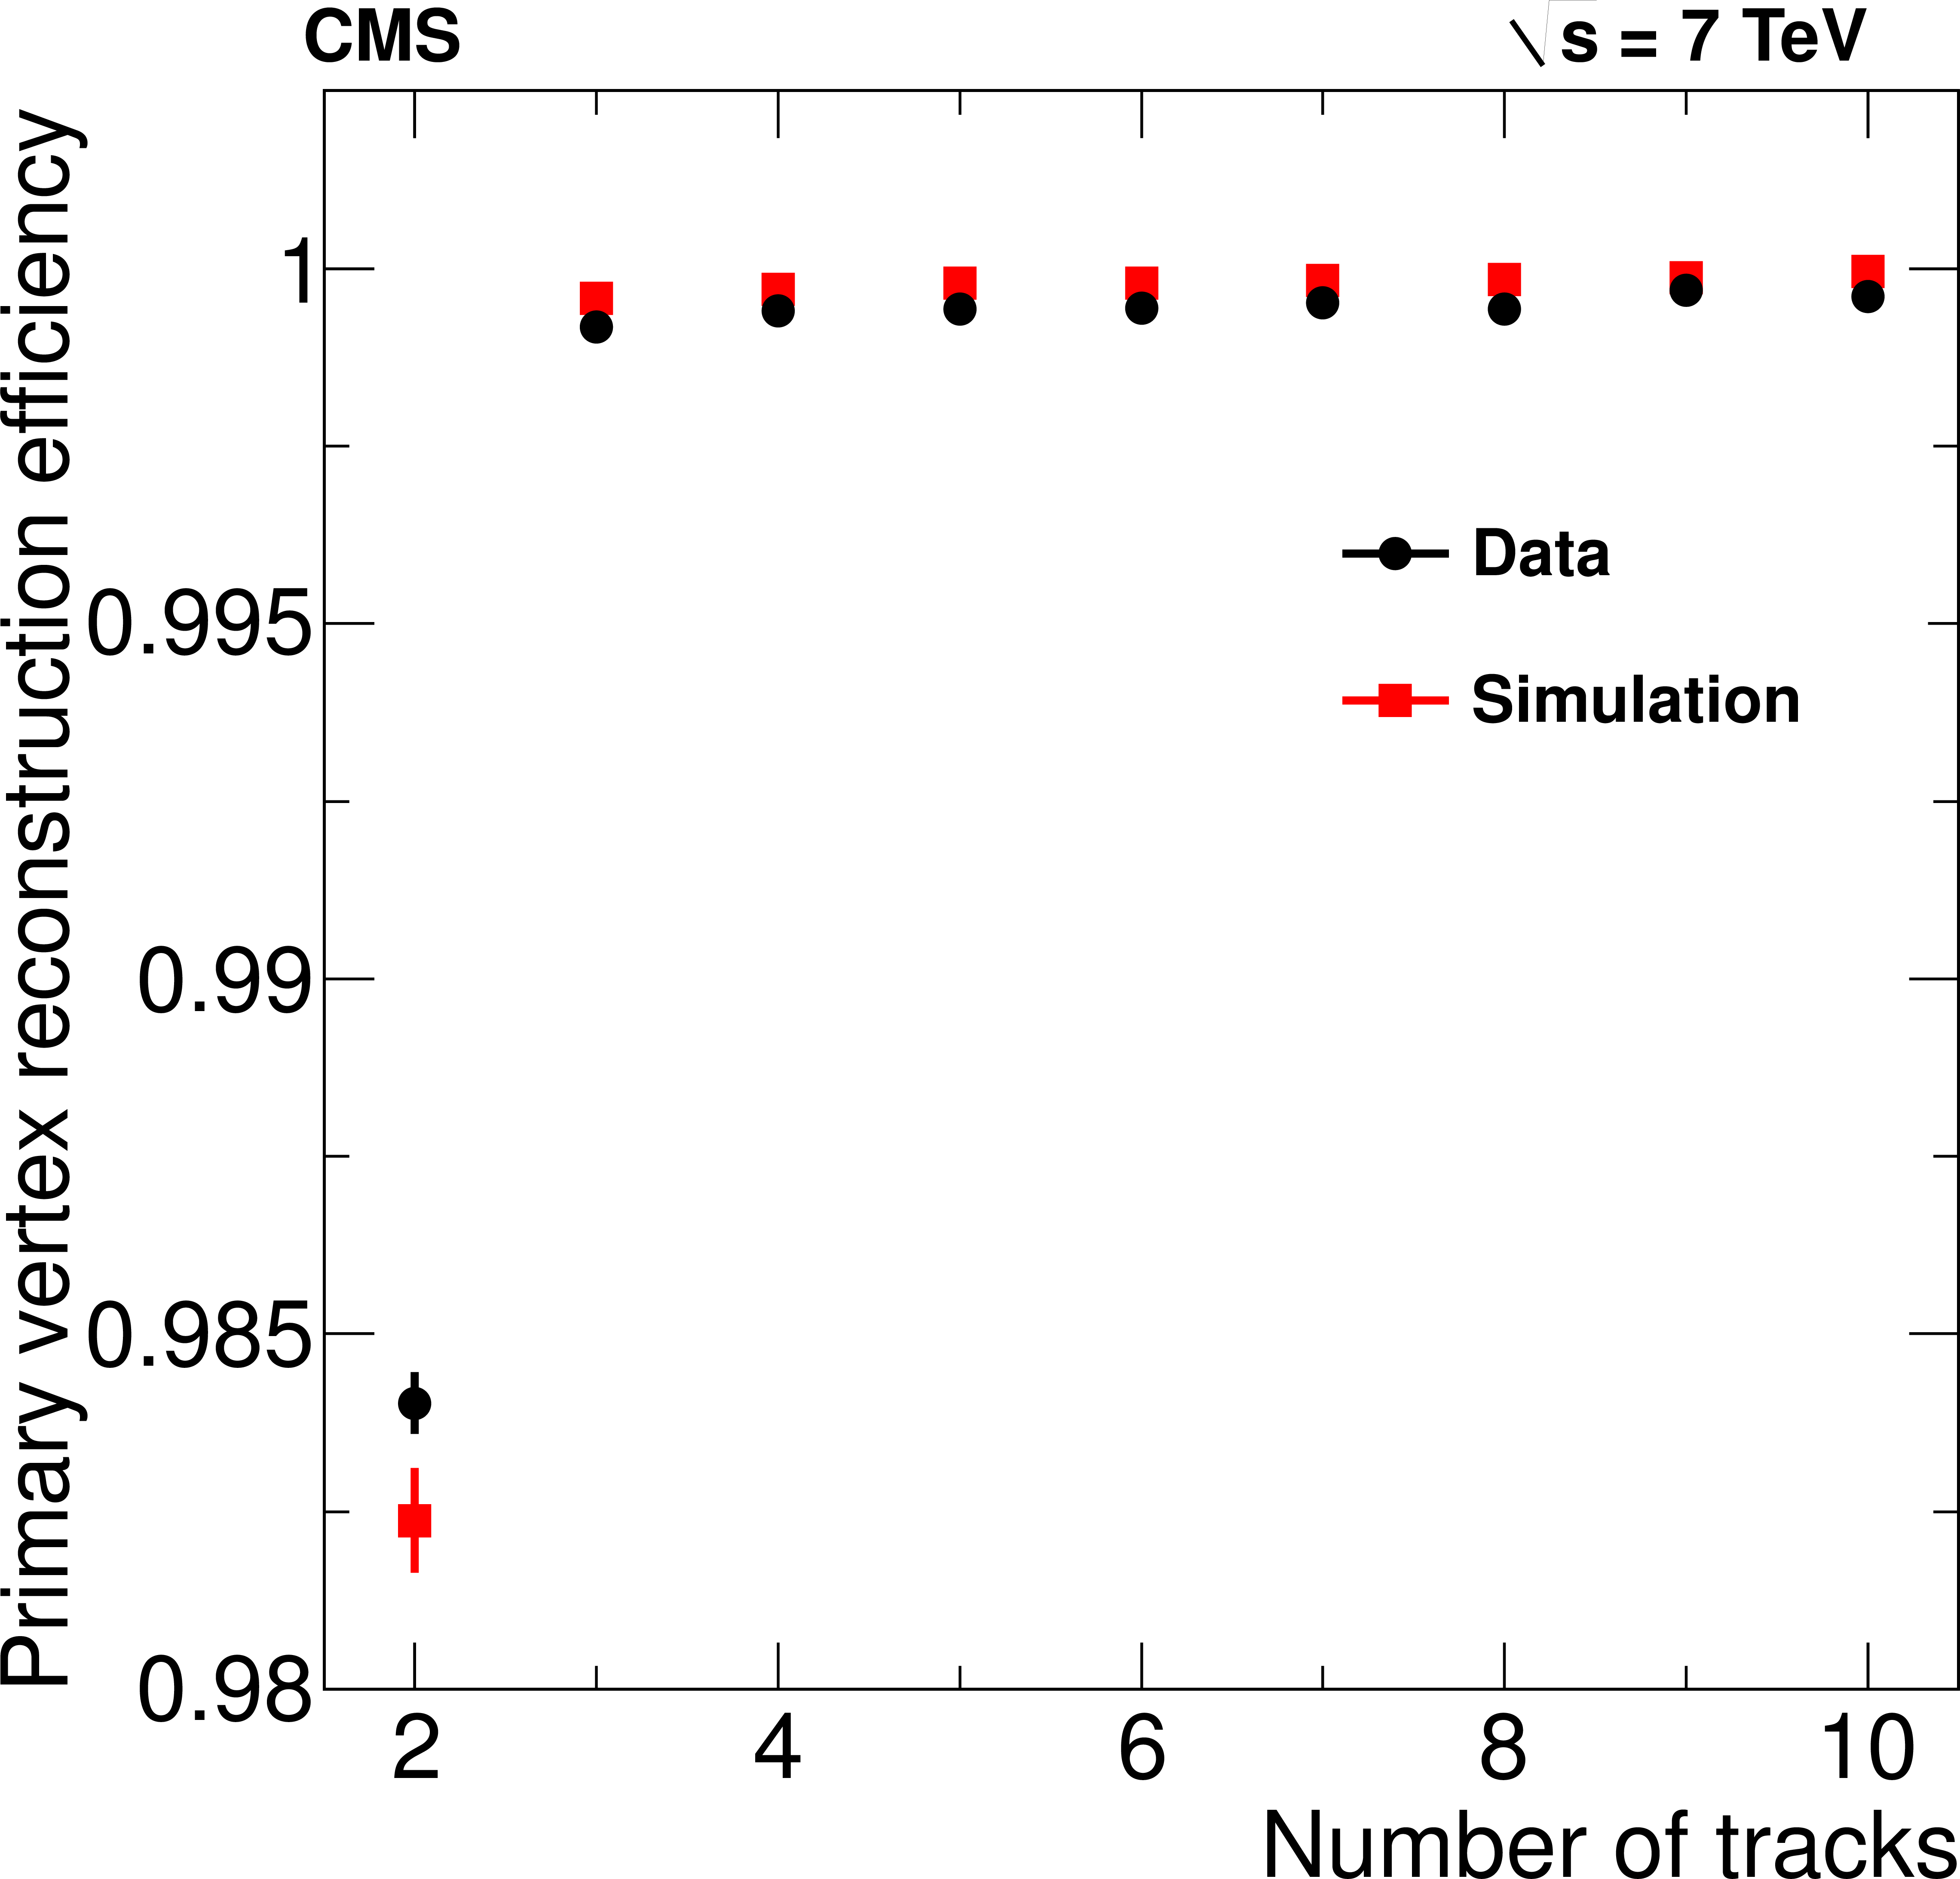
\includegraphics[width=0.49\columnwidth]{figures_chapter4/vertex_efficiency}
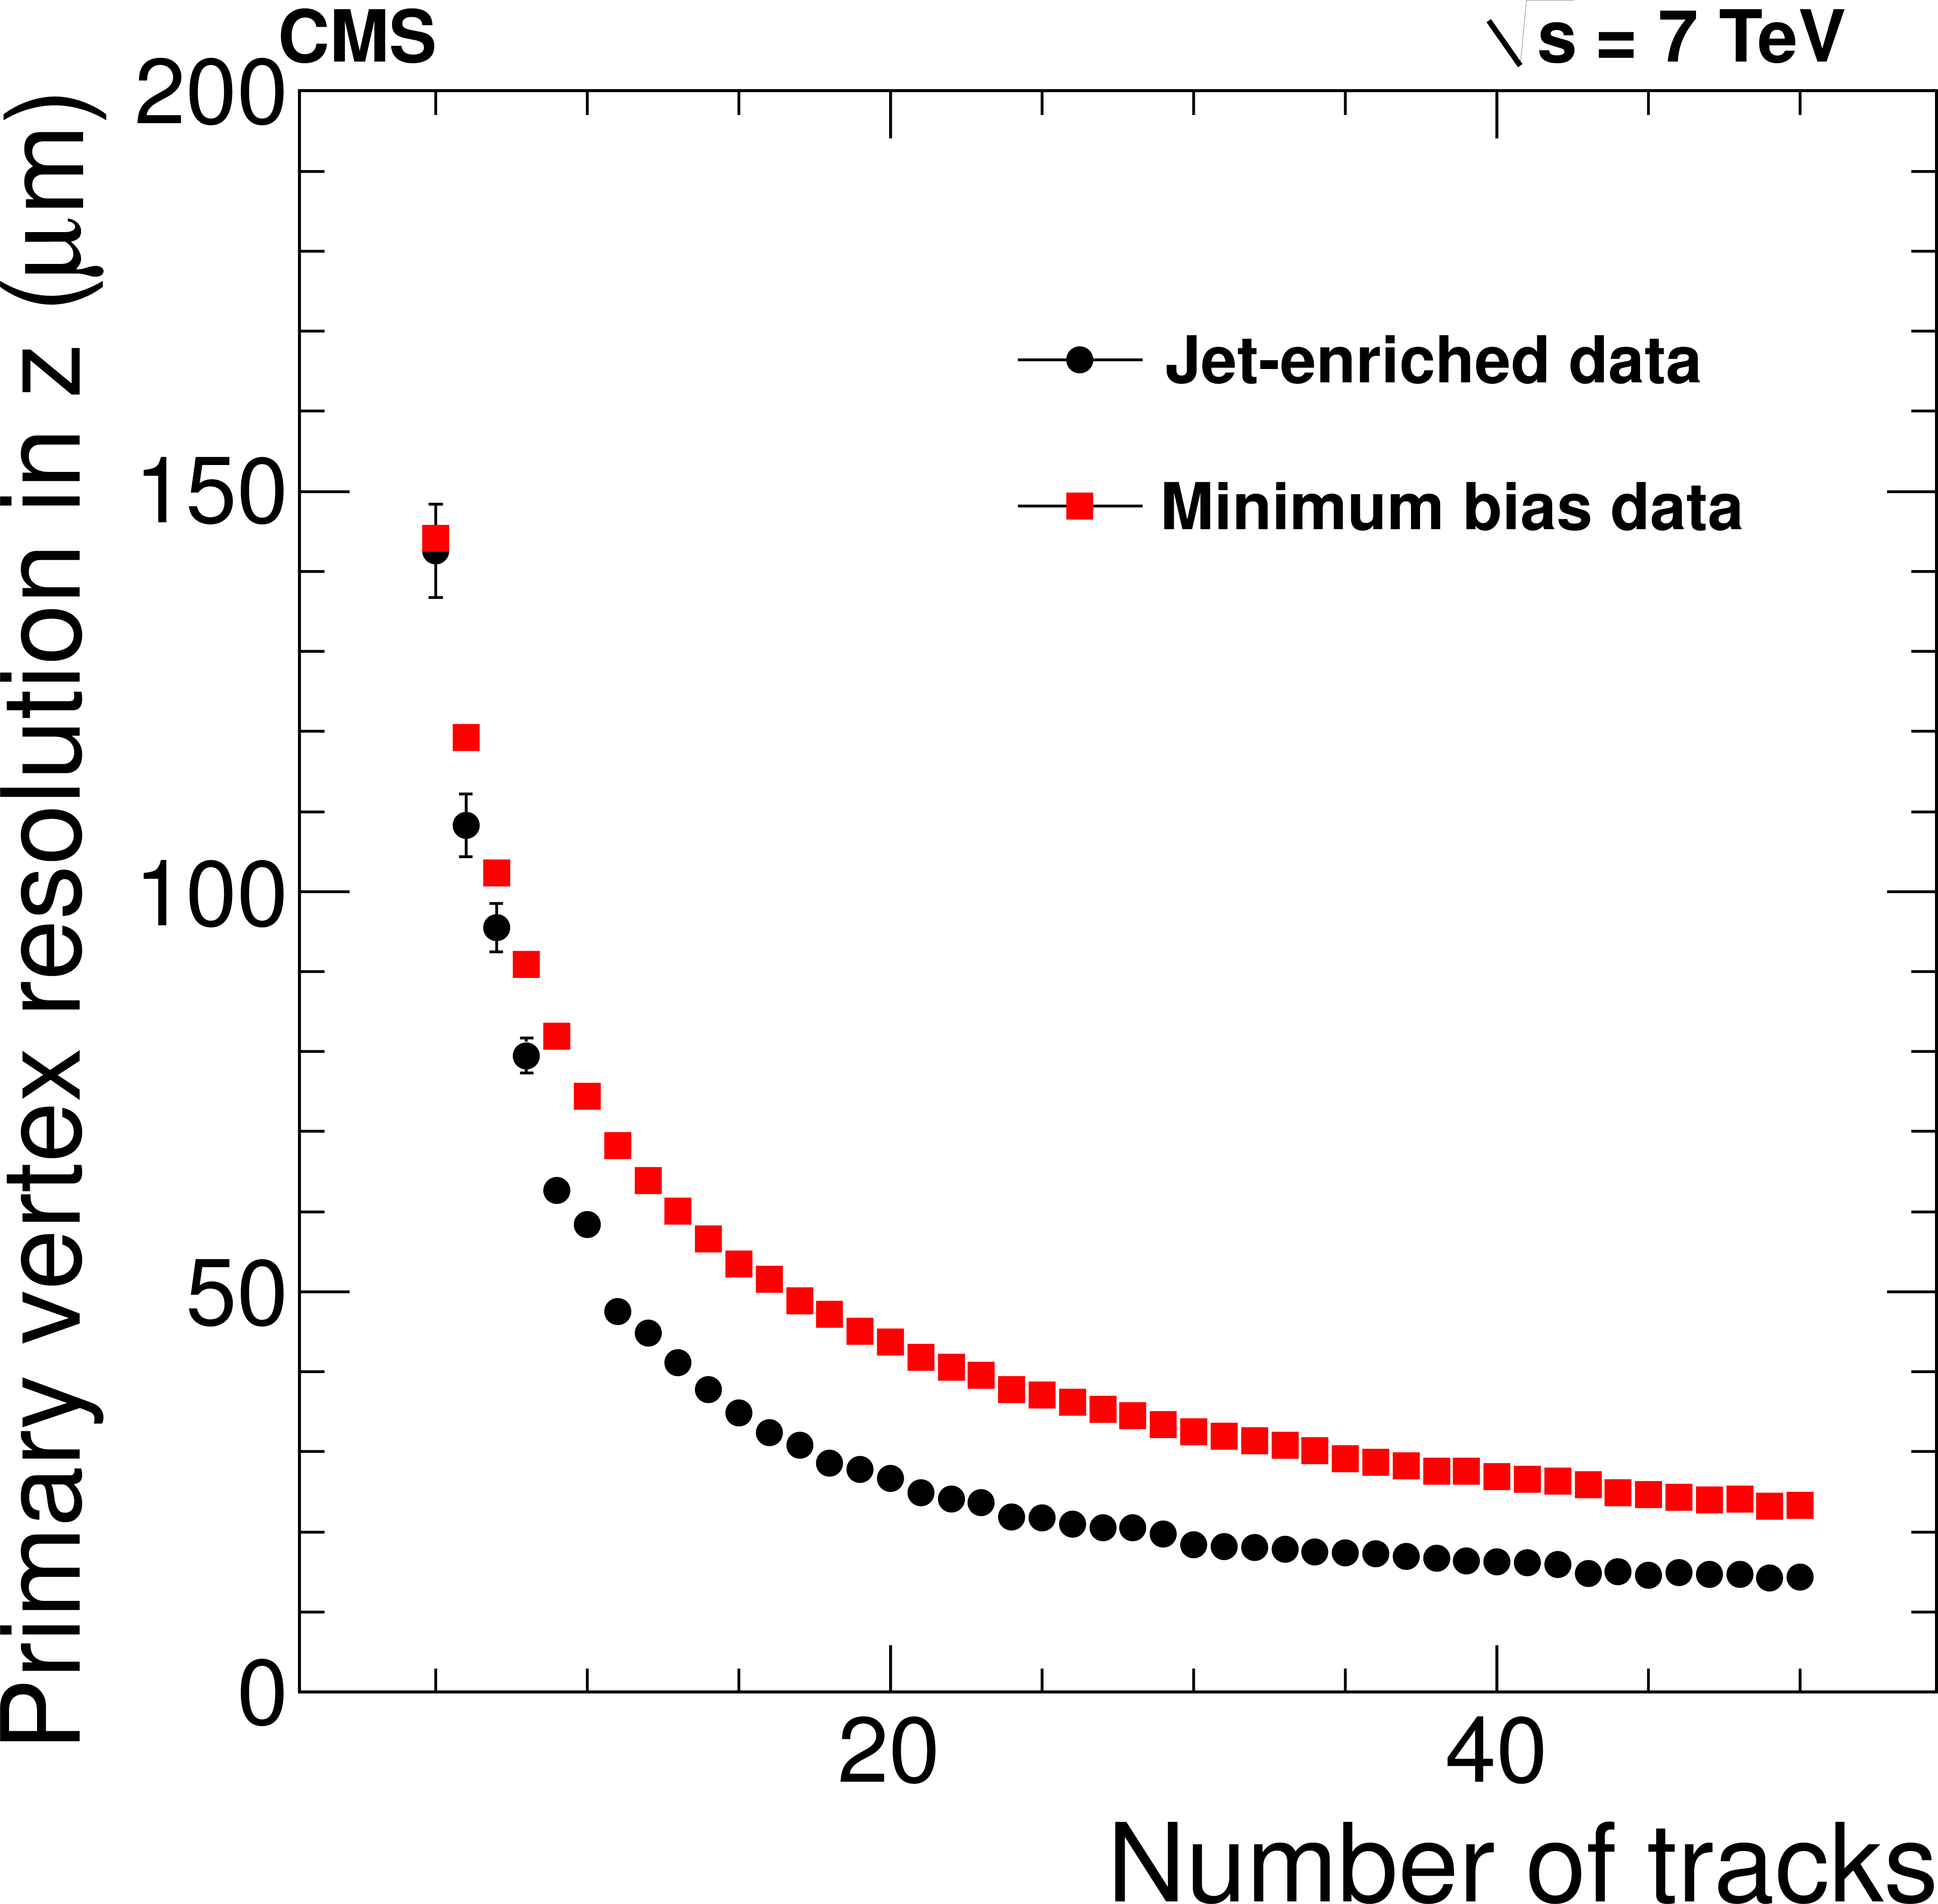
\includegraphics[width=0.49\columnwidth]{figures_chapter4/vertex_resolution}
\caption{Vertex reconstruction efficiency (left panel) as a function of the number of tracks in the vertex measured in minimum-bias data and in simulation. Vertex resolution (right panel) in the $z$ coordinate as a function of the number of tracks measured in minimum bias events (red) and jet-enriched events (black)~\cite{Chatrchyan:2014fea}.}
\label{fig:vertex}
\end{figure}

The candidate vertices determined by the DA clustering that contain at least two tracks are fitted using an adaptive vertex fitter~\cite{0954-3899-34-12-N01} to determine all the vertex parameters including the $x$, $y$, and $z$ positions. Figure~\ref{fig:vertex} shows the vertex reconstruction efficiency (left) and vertex resolution in $z$ coordinate as a function of the number of tracks used to fit the vertex. The reconstruction efficiency is close to $100\%$ when there are more than two tracks used to reconstruct the vertex. The vertex resolution also depends on the number of tracks as well as the $p_{T}$ of the tracks. The vertex resolutions are shown for minimum bias data events (red), where loose triggers select inelastic pp collisions with as little bias as possible, and jet enriched data events, where the events are required to have a reconstructed jet with transverse energy $E_{T}$ greater than $20~\GeV$ (black). The tracks in the jet enriched events have higher $p_{T}$ resulting in better vertex resolution. A resolution of approximately $10$ $\mu$m is achieved for high $p_{T}$ vertices with at least $50$ tracks.   

The vertex with the largest sum of the $p_{T}^2$ is defined to be the true hard-scattered pp vertex and is denoted as the primary vertex. The other vertices in the event are assumed to originate from the additional pileup interactions in the bunch crossing. Beam induced backgrounds can be rejected by applying compatibility requirements on the primary vertex with the nominal interaction point (the origin of the CMS coordinate system). The distance of the primary vertex in the $z$ direction (transverse direction) to the nominal interaction point is required to be less than $24$ cm ($2$ cm). The number of degrees of freedom of the primary vertex fit is also required to be greater than $3$.

\section{Muon Reconstruction}

Muon tracks are reconstructed not only in the CMS inner tracker but also independently in the muon system~\cite{Chatrchyan:2012xi}. The latter tracks are called standalone muon tracks. The standalone muon tracks are reconstructed from the hits in the muon chambers in a combined track fit using a Kalman filter. The "global muon" reconstruction refers to the combination and matching of the standalone muon tracks with the inner tracker tracks. A global muon track is fitted from these tracks again using a Kalman filter technique. The expected energy loss in the solenoid and support structures is taken into account in the fit. The global fit improves the momentum resolution for muons with $p_{T}$ greater than $200~\GeV$ compared to the inner tracker only resolution as demonstrated in Figure~\ref{fig:muon_resolution}.   

Another independent algorithm starts from the inner tracker and proceeds outward in the radial direction matching the hits in the muons chambers. These "tracker muon" reconstruction is more efficient for low momentum muons ($p < 5~\GeV$) compared to the global muon reconstruction as it only requires one muon segment hit in the muon chambers. The tracker muon reconstruction considers all the inner tracker tracks with $p_{T}$ greater than $0.5~\GeV$ as possible muon candidates. The average expected energy loses and multiple Coulomb scattering in the detector material are taken into account for the extrapolation to the muon system. 

\begin{figure}[h]
\centering
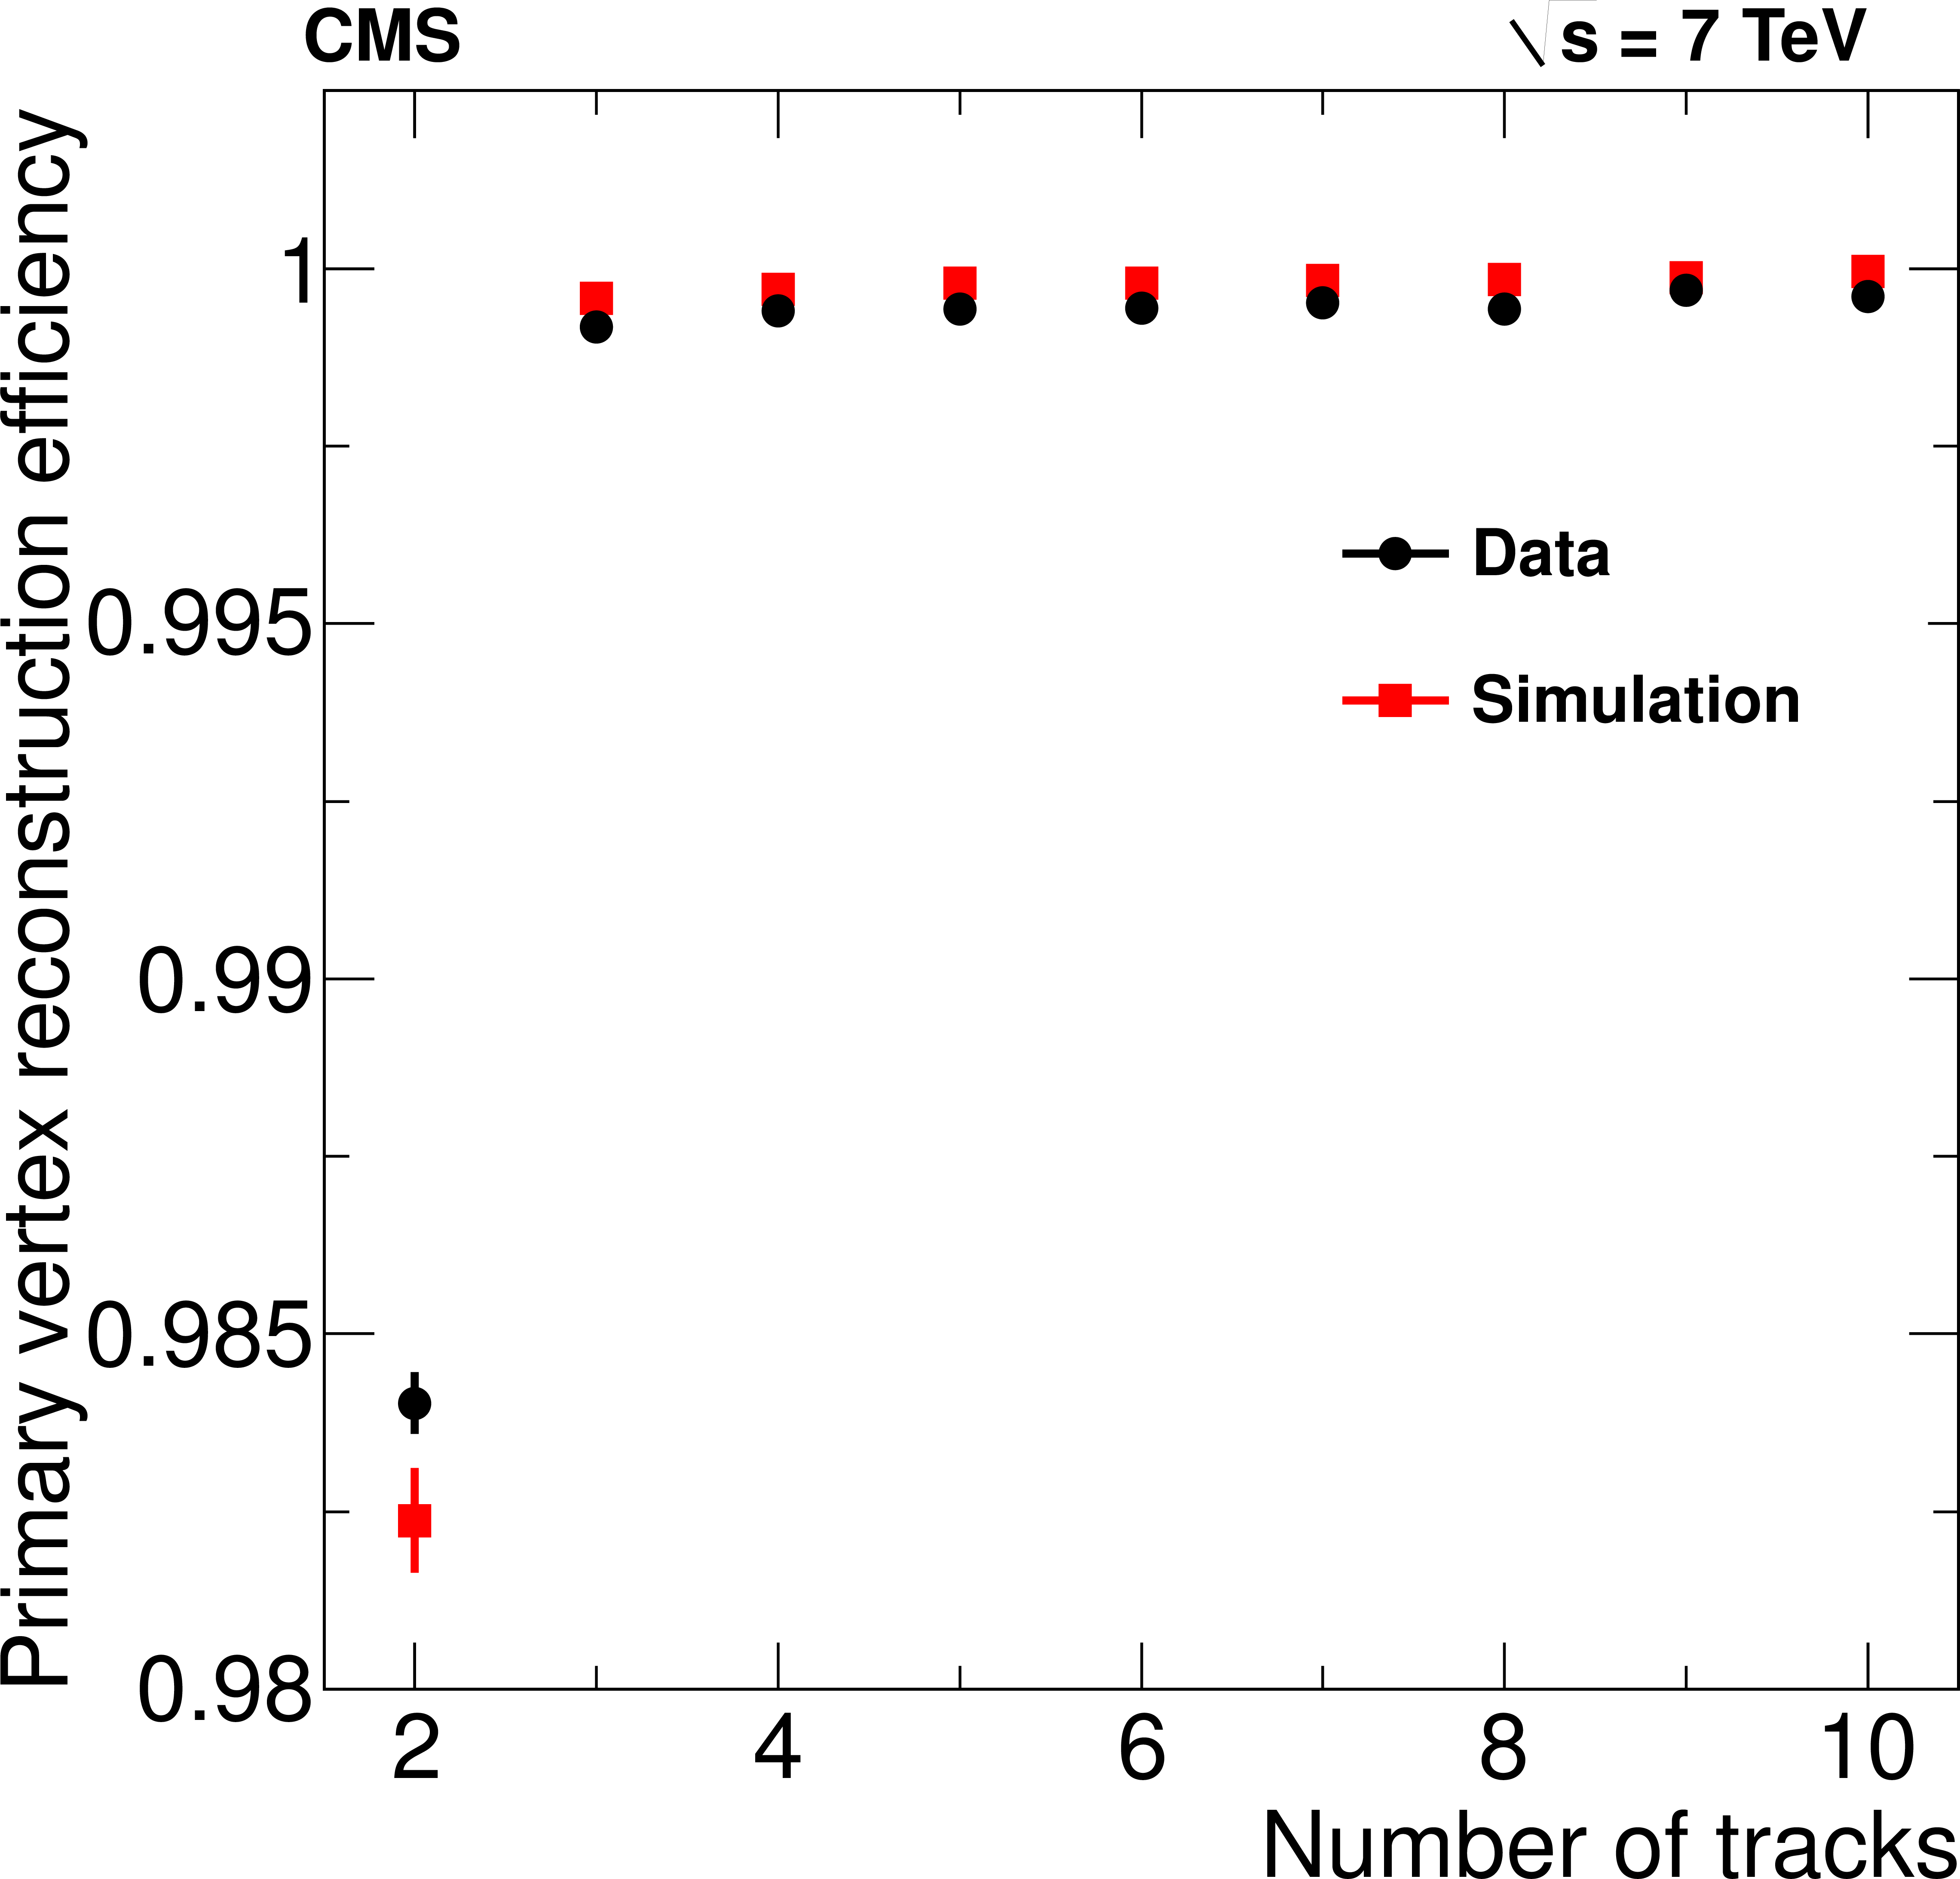
\includegraphics[width=0.35\columnwidth]{figures_chapter4/vertex_efficiency}
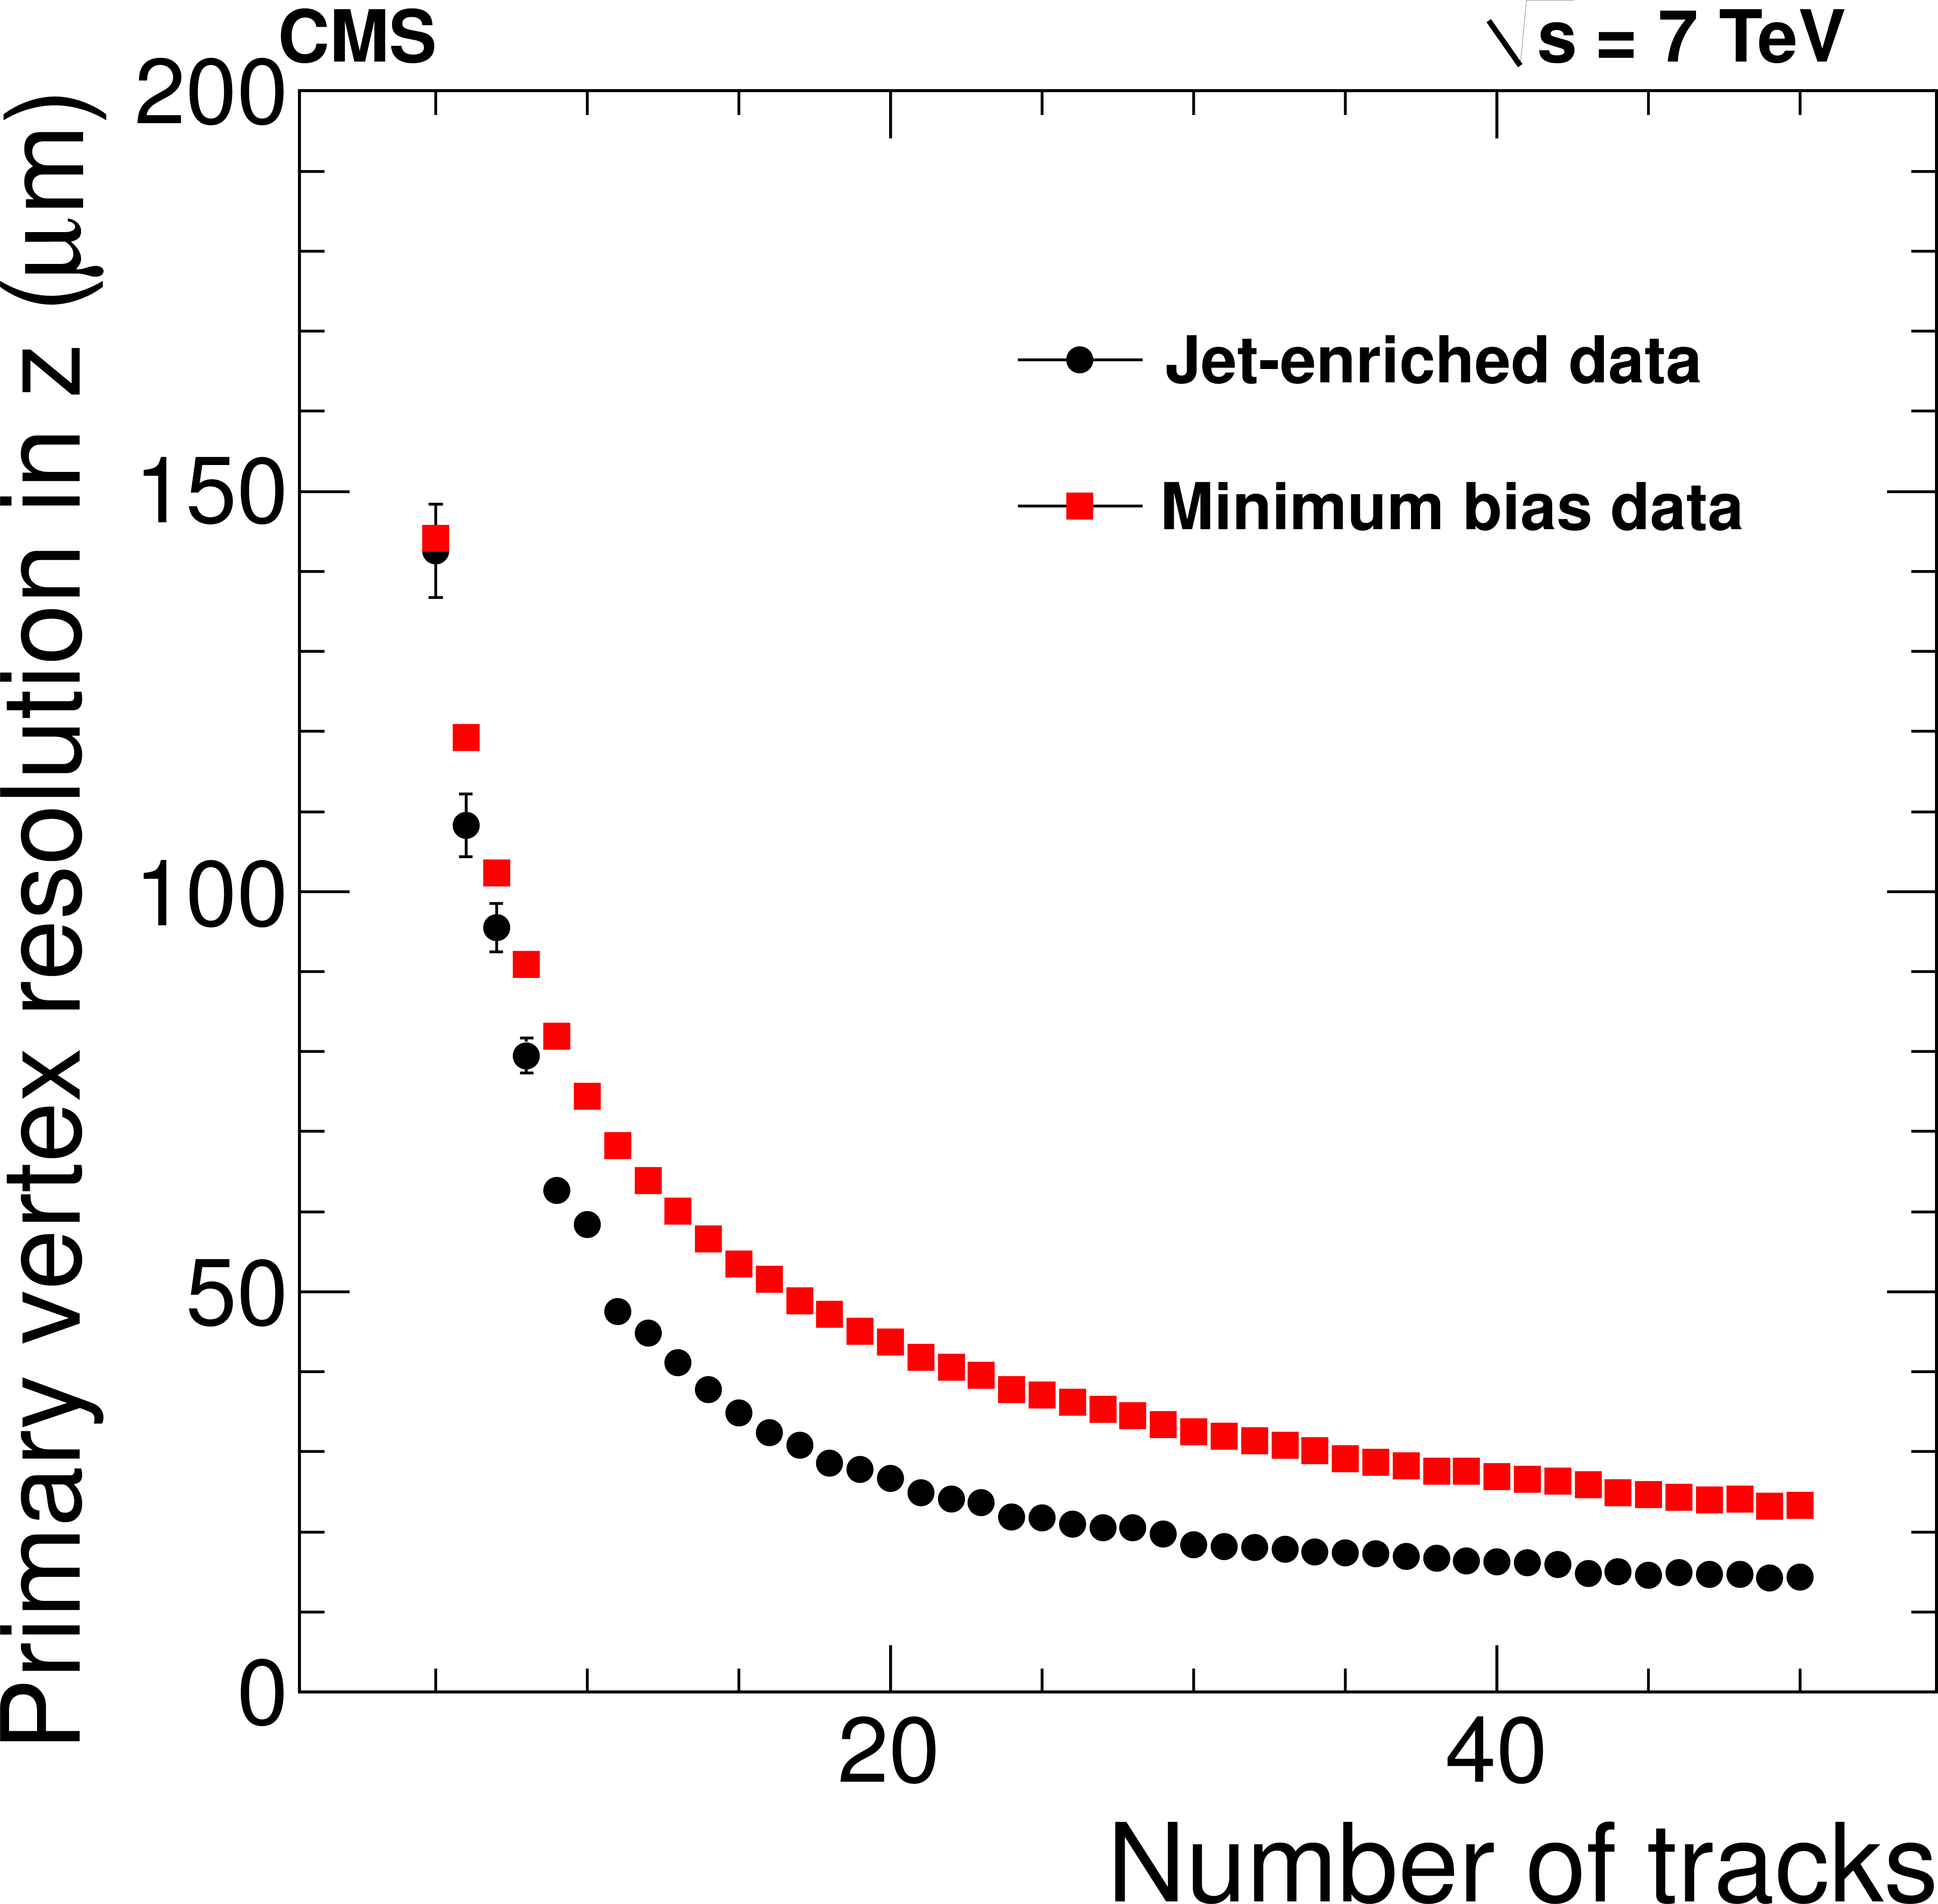
\includegraphics[width=0.35\columnwidth]{figures_chapter4/vertex_resolution}
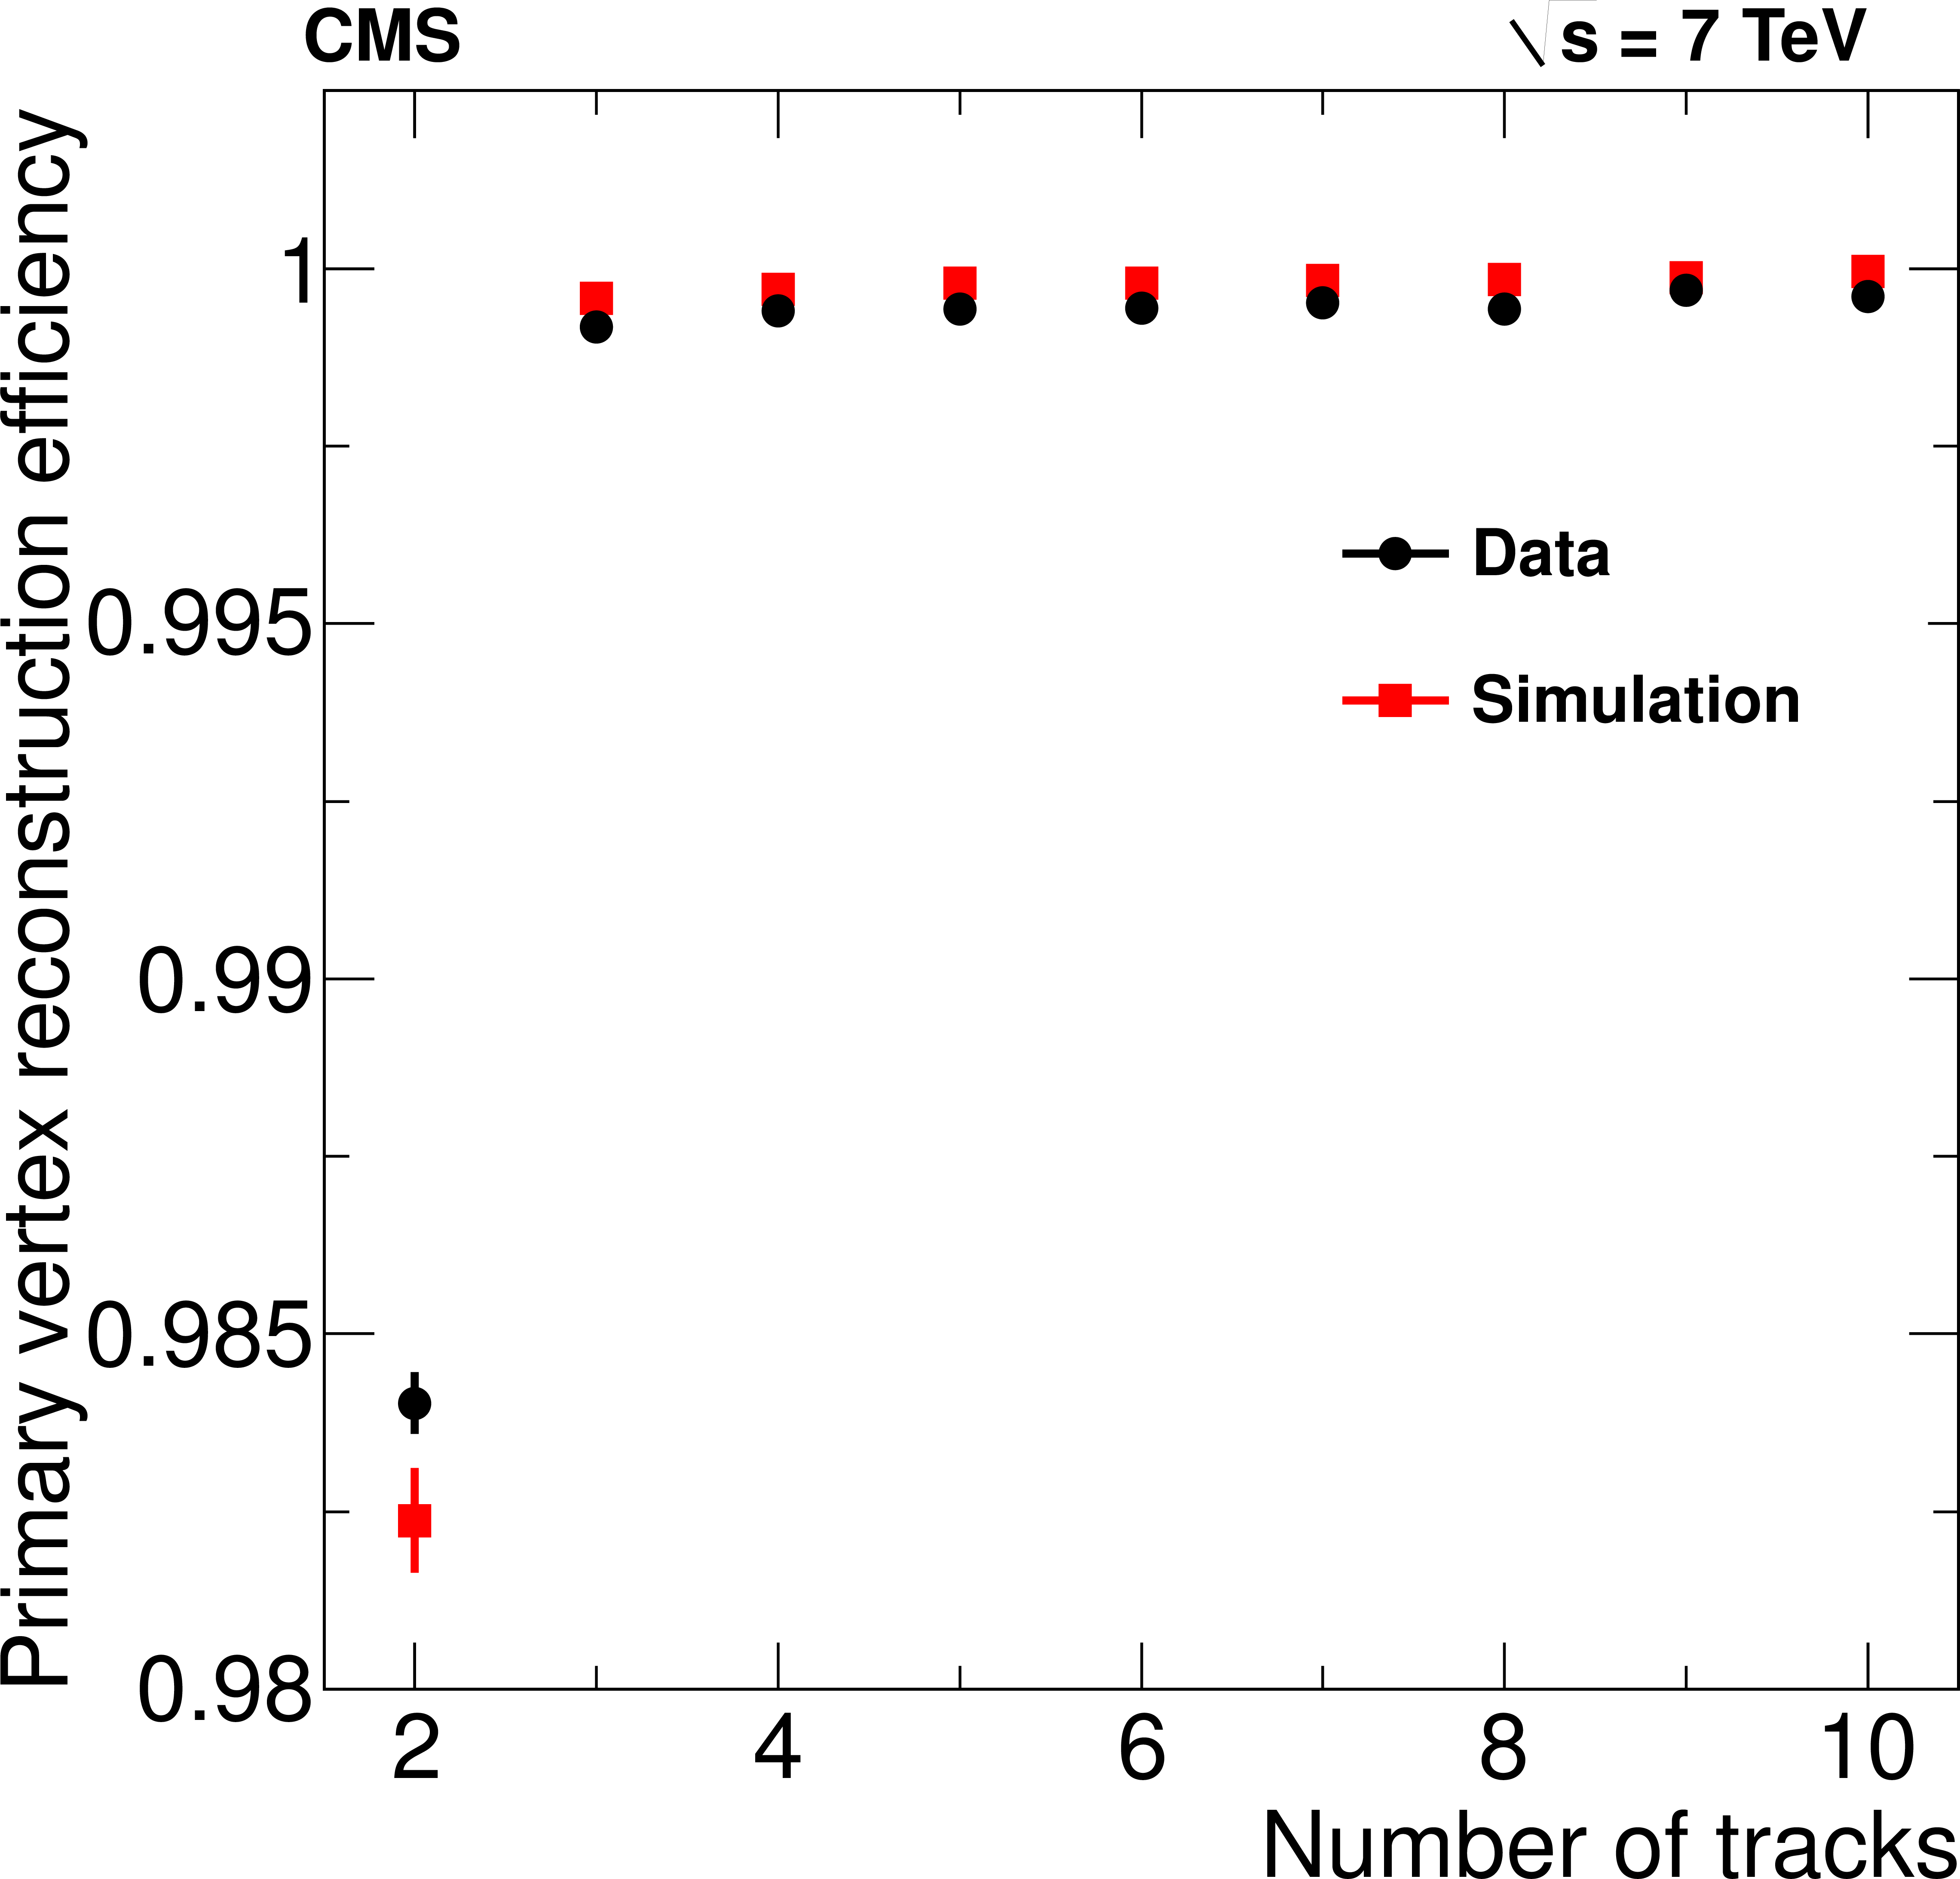
\includegraphics[width=0.35\columnwidth]{figures_chapter4/vertex_efficiency}
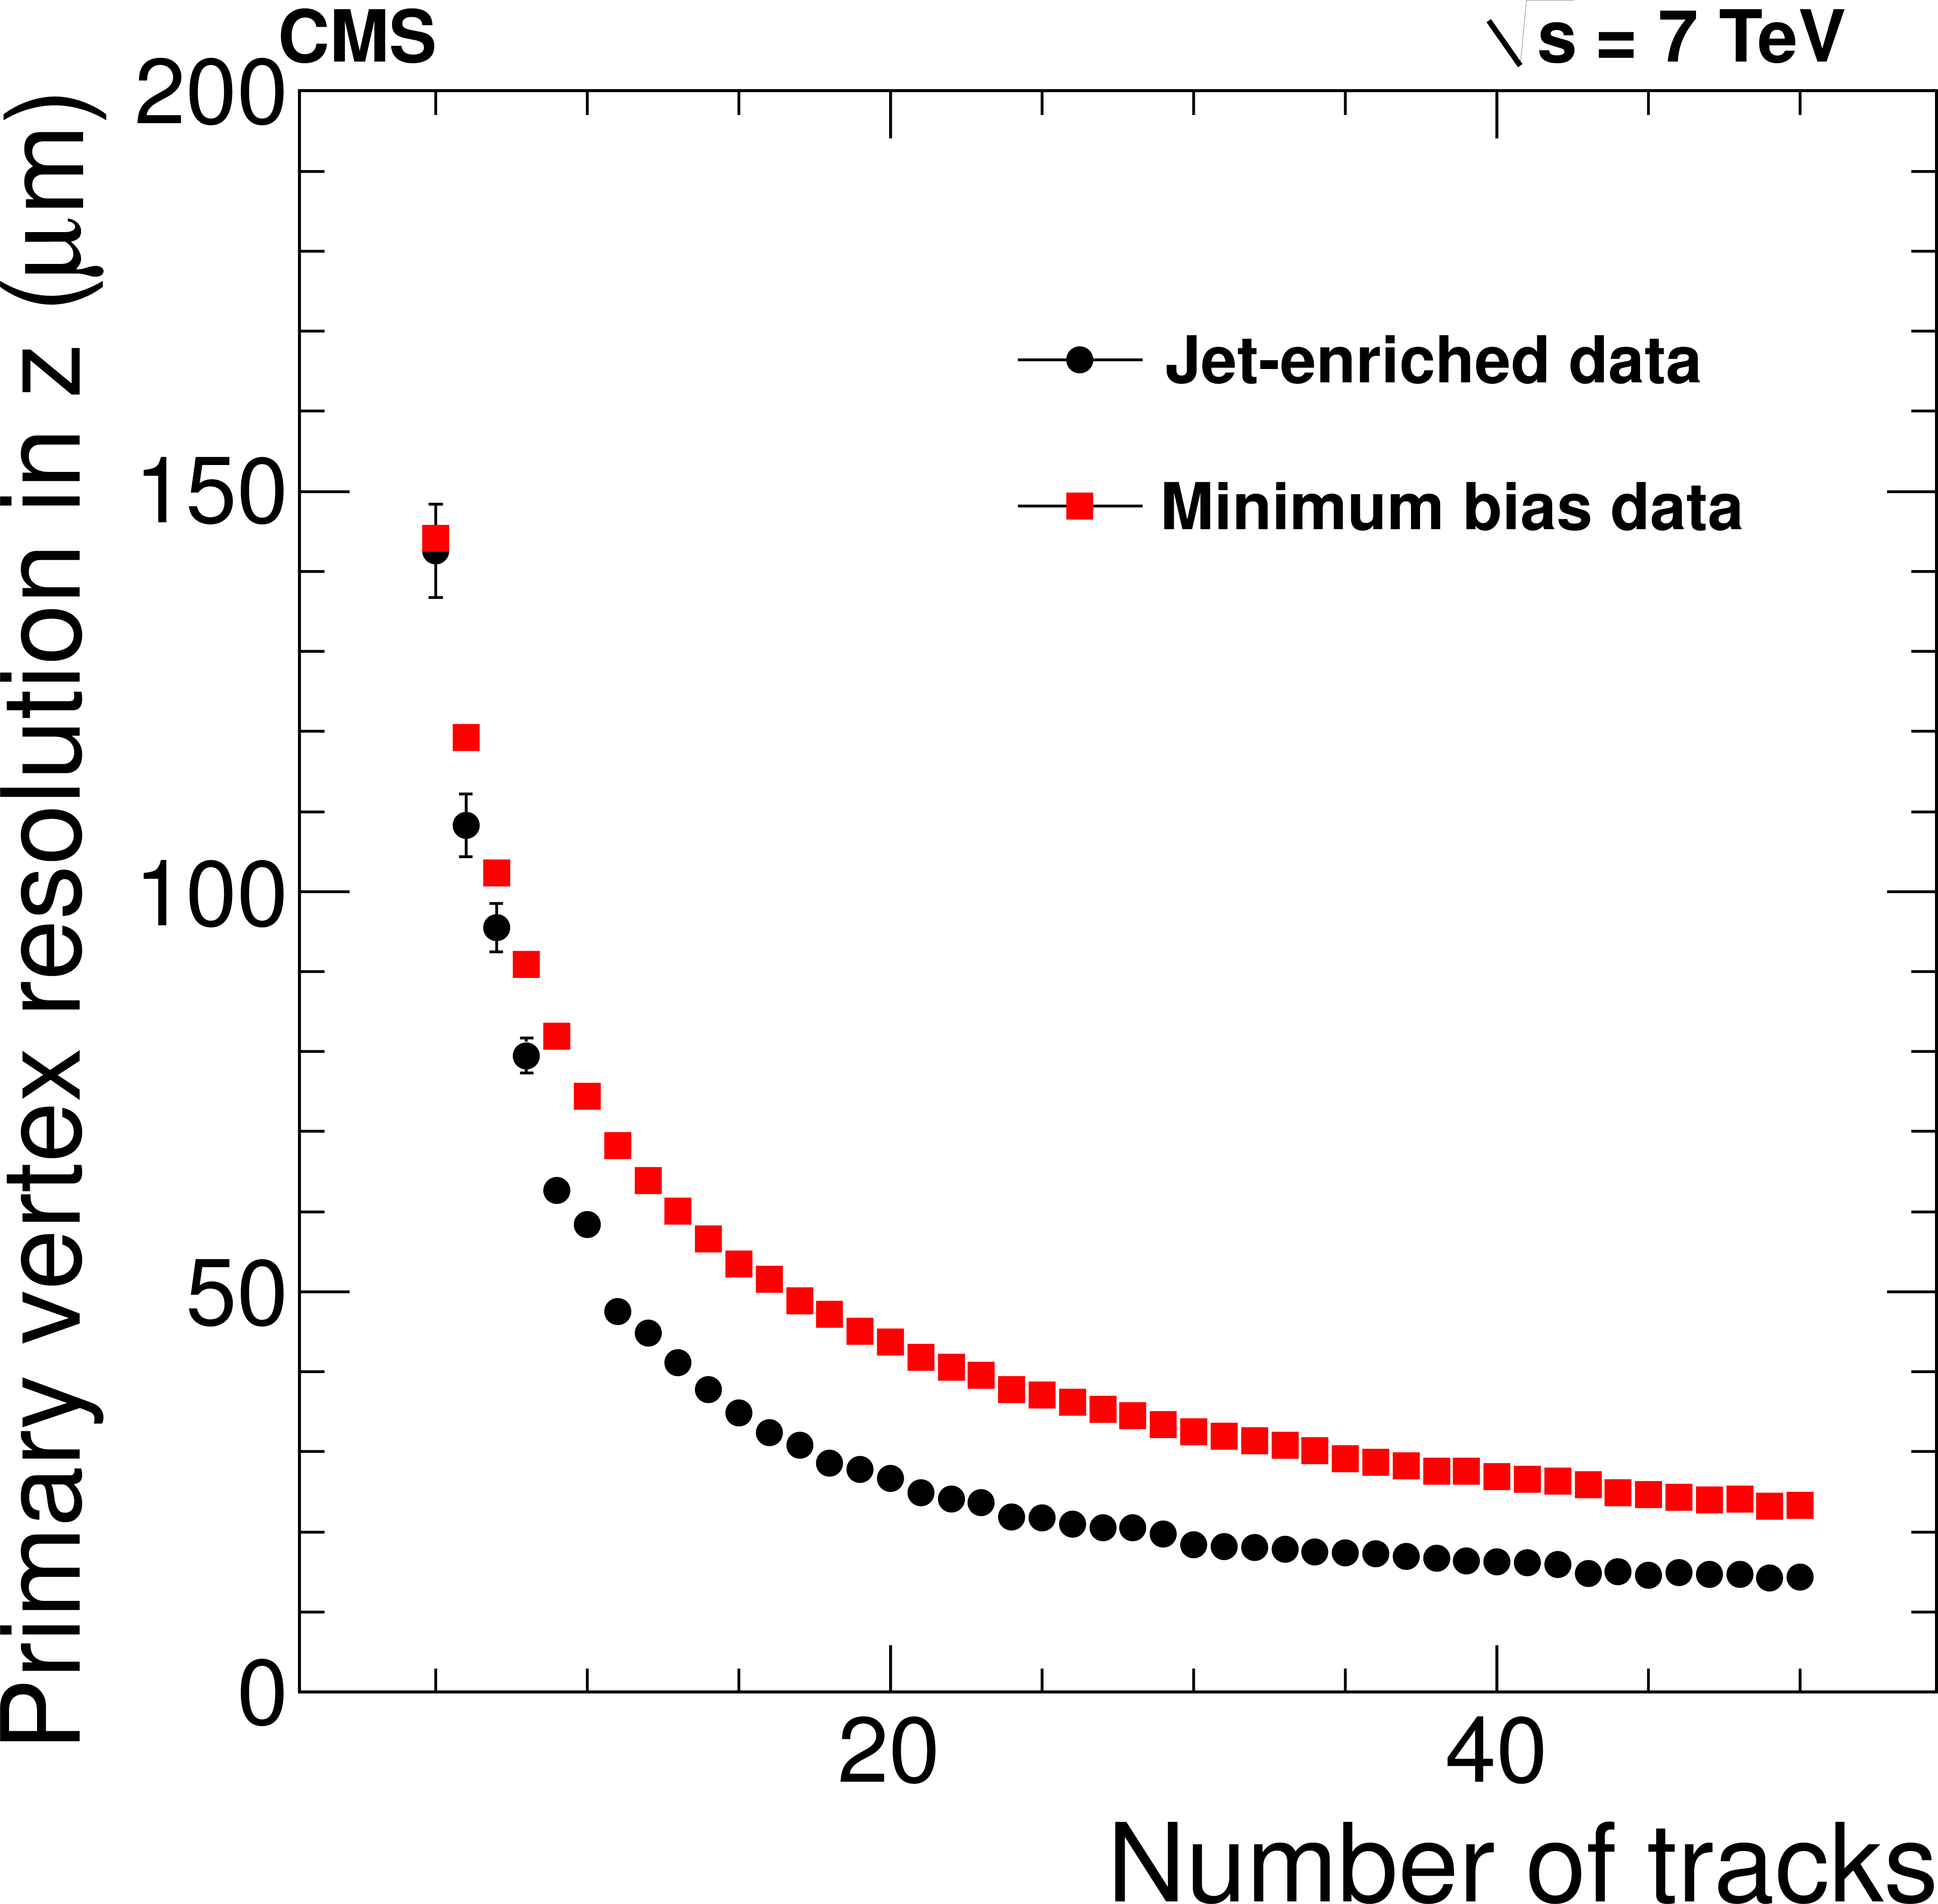
\includegraphics[width=0.35\columnwidth]{figures_chapter4/vertex_resolution}
\caption{Distribution of $\chi^2$ per degree of freedom, transverse impact parameter $d_{xy}$,  number of hits in the inner tracker, and number of muon station for data at $\sqrt{s}=13~\TeV$ taken during $2015$ data taking period. Simulated $W \rightarrow \mu \nu$ signal process normalized to the number of observed data evens is shown for comparison. The events satisfy all other selection requirements (including the isolation requirement to be discussed in chapter $4$) are satisfied except that on the shown variable.}
\label{fig:muon_id}
\end{figure}

Muon candidates selected in the results are required to be either a tracker or a global muon. Approximately $99\%$ of the muons in the fiducial volume (the geometrical acceptance) of the muon system are identified as either a tracker or a global muon. Muon candidates identified as both a global and a tracker muon are merged into a single candidate.  Additional quality requirements are imposed to reduce miss-identified muon candidates and so called non-prompt muons. Non-prompt muons originate from in-flight decays of light hadrons and semi-leptonic decays of the heavy flavor quarks. The miss-identified muon candidates originate from the punch-through of hadronic showers to the muon system. The contribution is generally small for the global muons due to the minimum number number of muon segment hits requirement. 

Figure~\ref{fig:muon_id} shows the distributions of few of the muon variables used for reduction of the non-prompt and miss-identified muons. The  $\chi^2$ per degree of freedom of the global track fit is required to be less than $10$. At least one segment in the muon stations must be included in the global fit to reduce the punch-through hadrons. The muons are required to have track segments in at least two muon stations. At least one hit in the pixel tracker and at least five tracking layers are required. Background originating from cosmic-ray muons transversing the CMS detector in coincidence with a pp collision is reduced by the impact parameter requirement. Figure~\ref{fig:muon_id} (up right) shows the transverse impact parameter distribution $d_{xy}$. The candidates with large $d_{xy}$ originate mainly from the cosmic-ray muons.  The excess of events with respect to the $W \rightarrow \mu\nu$ simulation is due to the in-flight decays of long lived particles in the QCD multi-jet background. 

\section{Electron Reconstruction}

Electrons are reconstructed by looking for a track in the inner tracking that is matched to energy deposits in the ECAL. Electron reconstruction is complicated due to bremsstrahlung radiation as electrons transverse the inner tracker detector. These bremsstrahlung photons can subsequently undergo a pair-conversion before reaching the ECAL. As a result the electron energy reaching the ECAL significantly spread in the azimuthal direction $\phi$ due to bending of the trajectories in the CMS magnetic field. Approximately $35\%$ of electrons radiate moe than $70\%$ of their initial energy before reaching the ECAL~\cite{Chatrchyan:2014fea,Baffioni:2006cd}. As a result a dedicated clustering algorithms are used to collect the bremsstrahlung energy taking the spreading in the $\phi$ direction into account~\cite{Meschi:2001lfa}.  The spread in the $\eta$ direction is mostly negligible except for very low $p_{T}$ (less than $5~\GeV$).    

\begin{figure}[h]
\centering
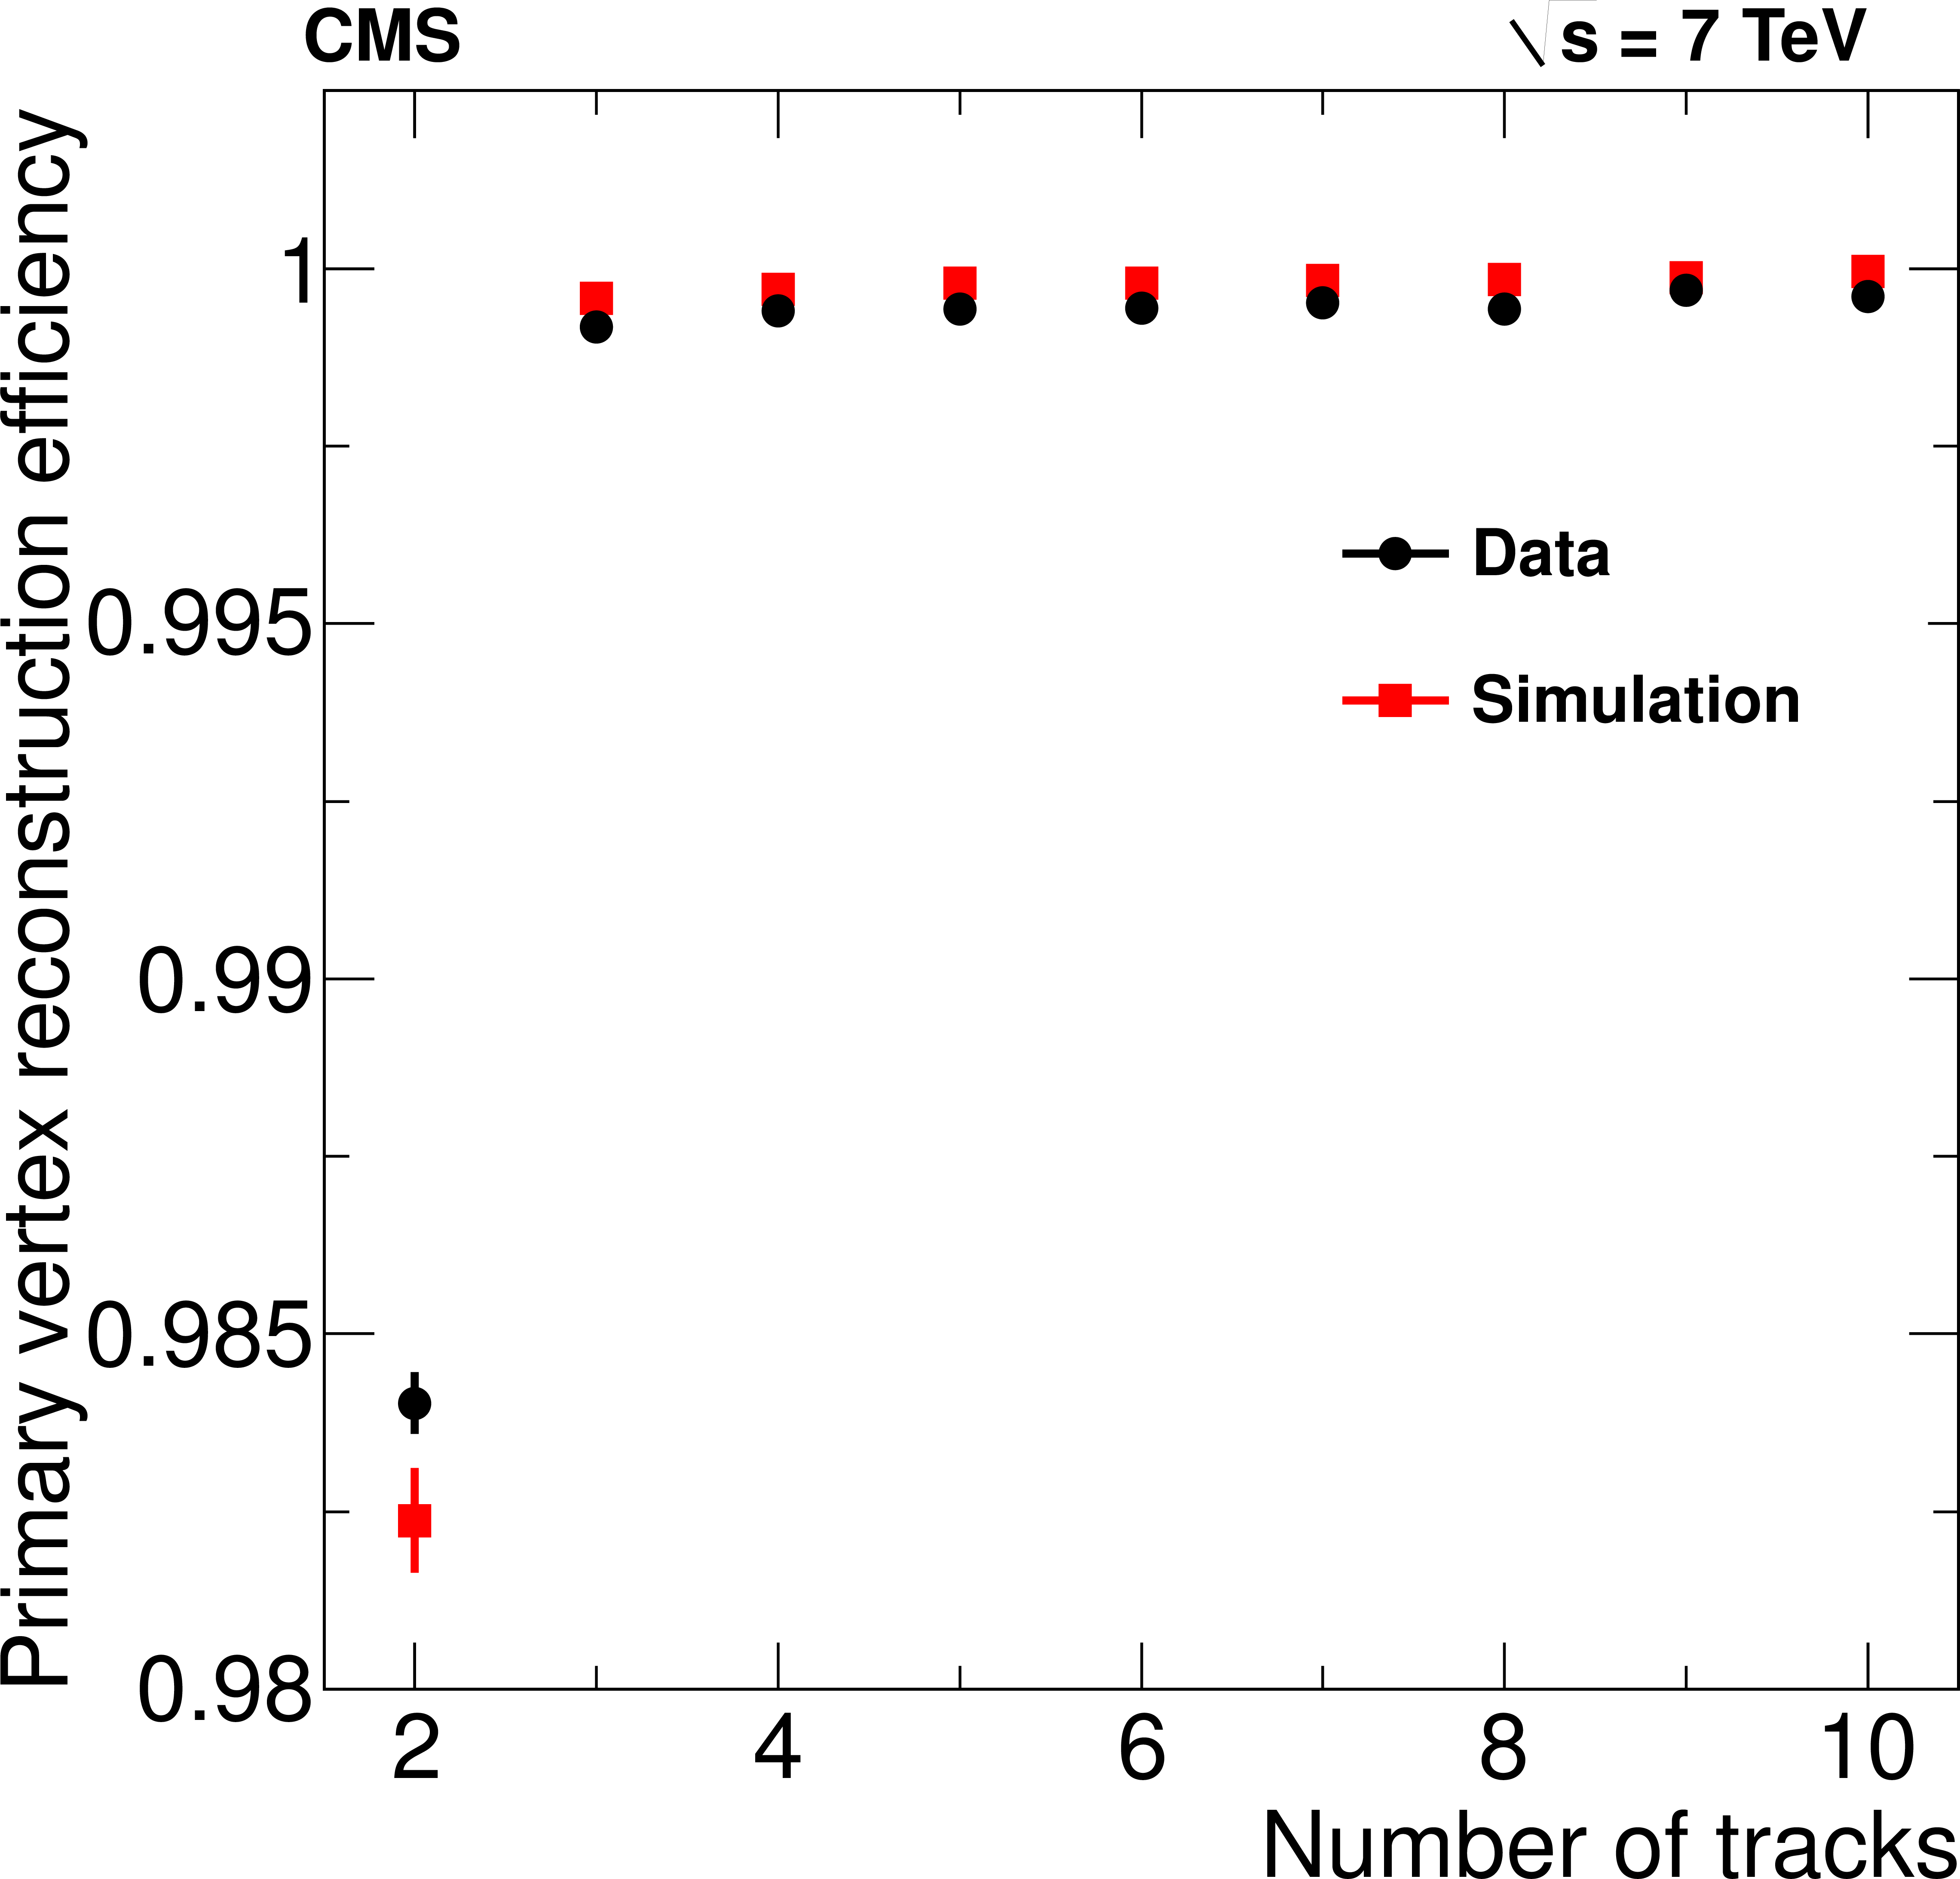
\includegraphics[width=0.32\columnwidth]{figures_chapter4/vertex_efficiency}
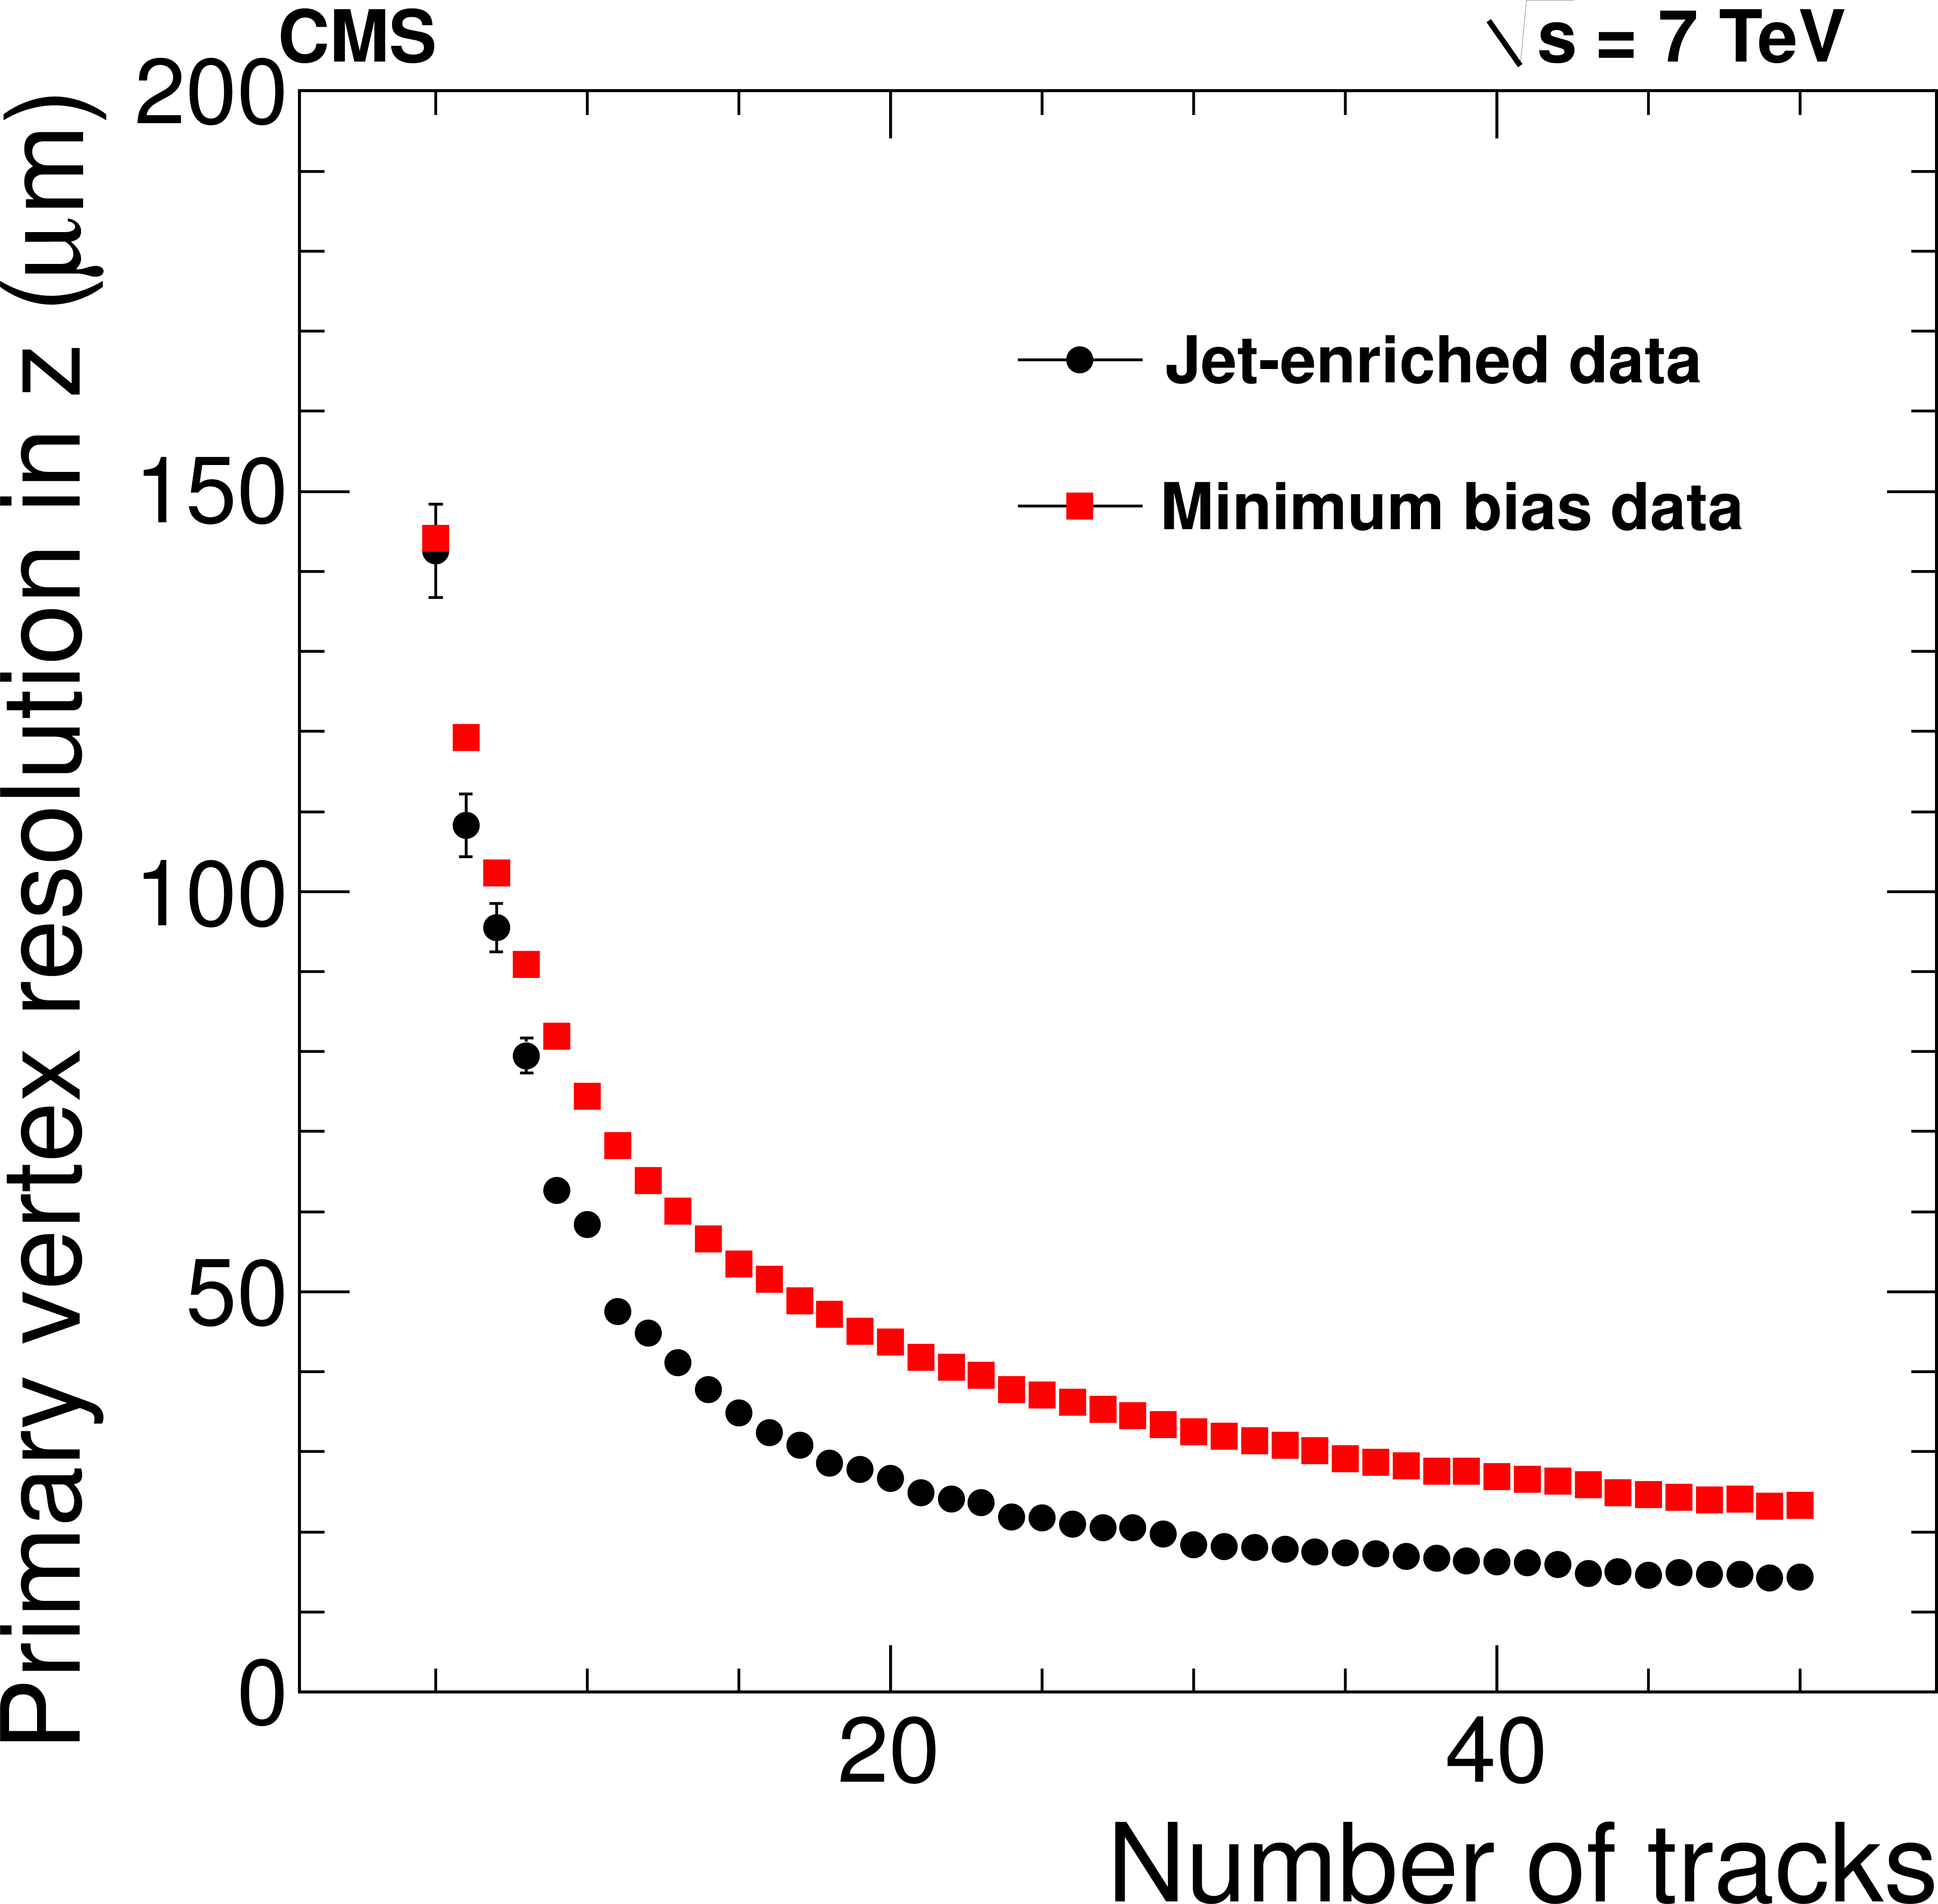
\includegraphics[width=0.32\columnwidth]{figures_chapter4/vertex_resolution}
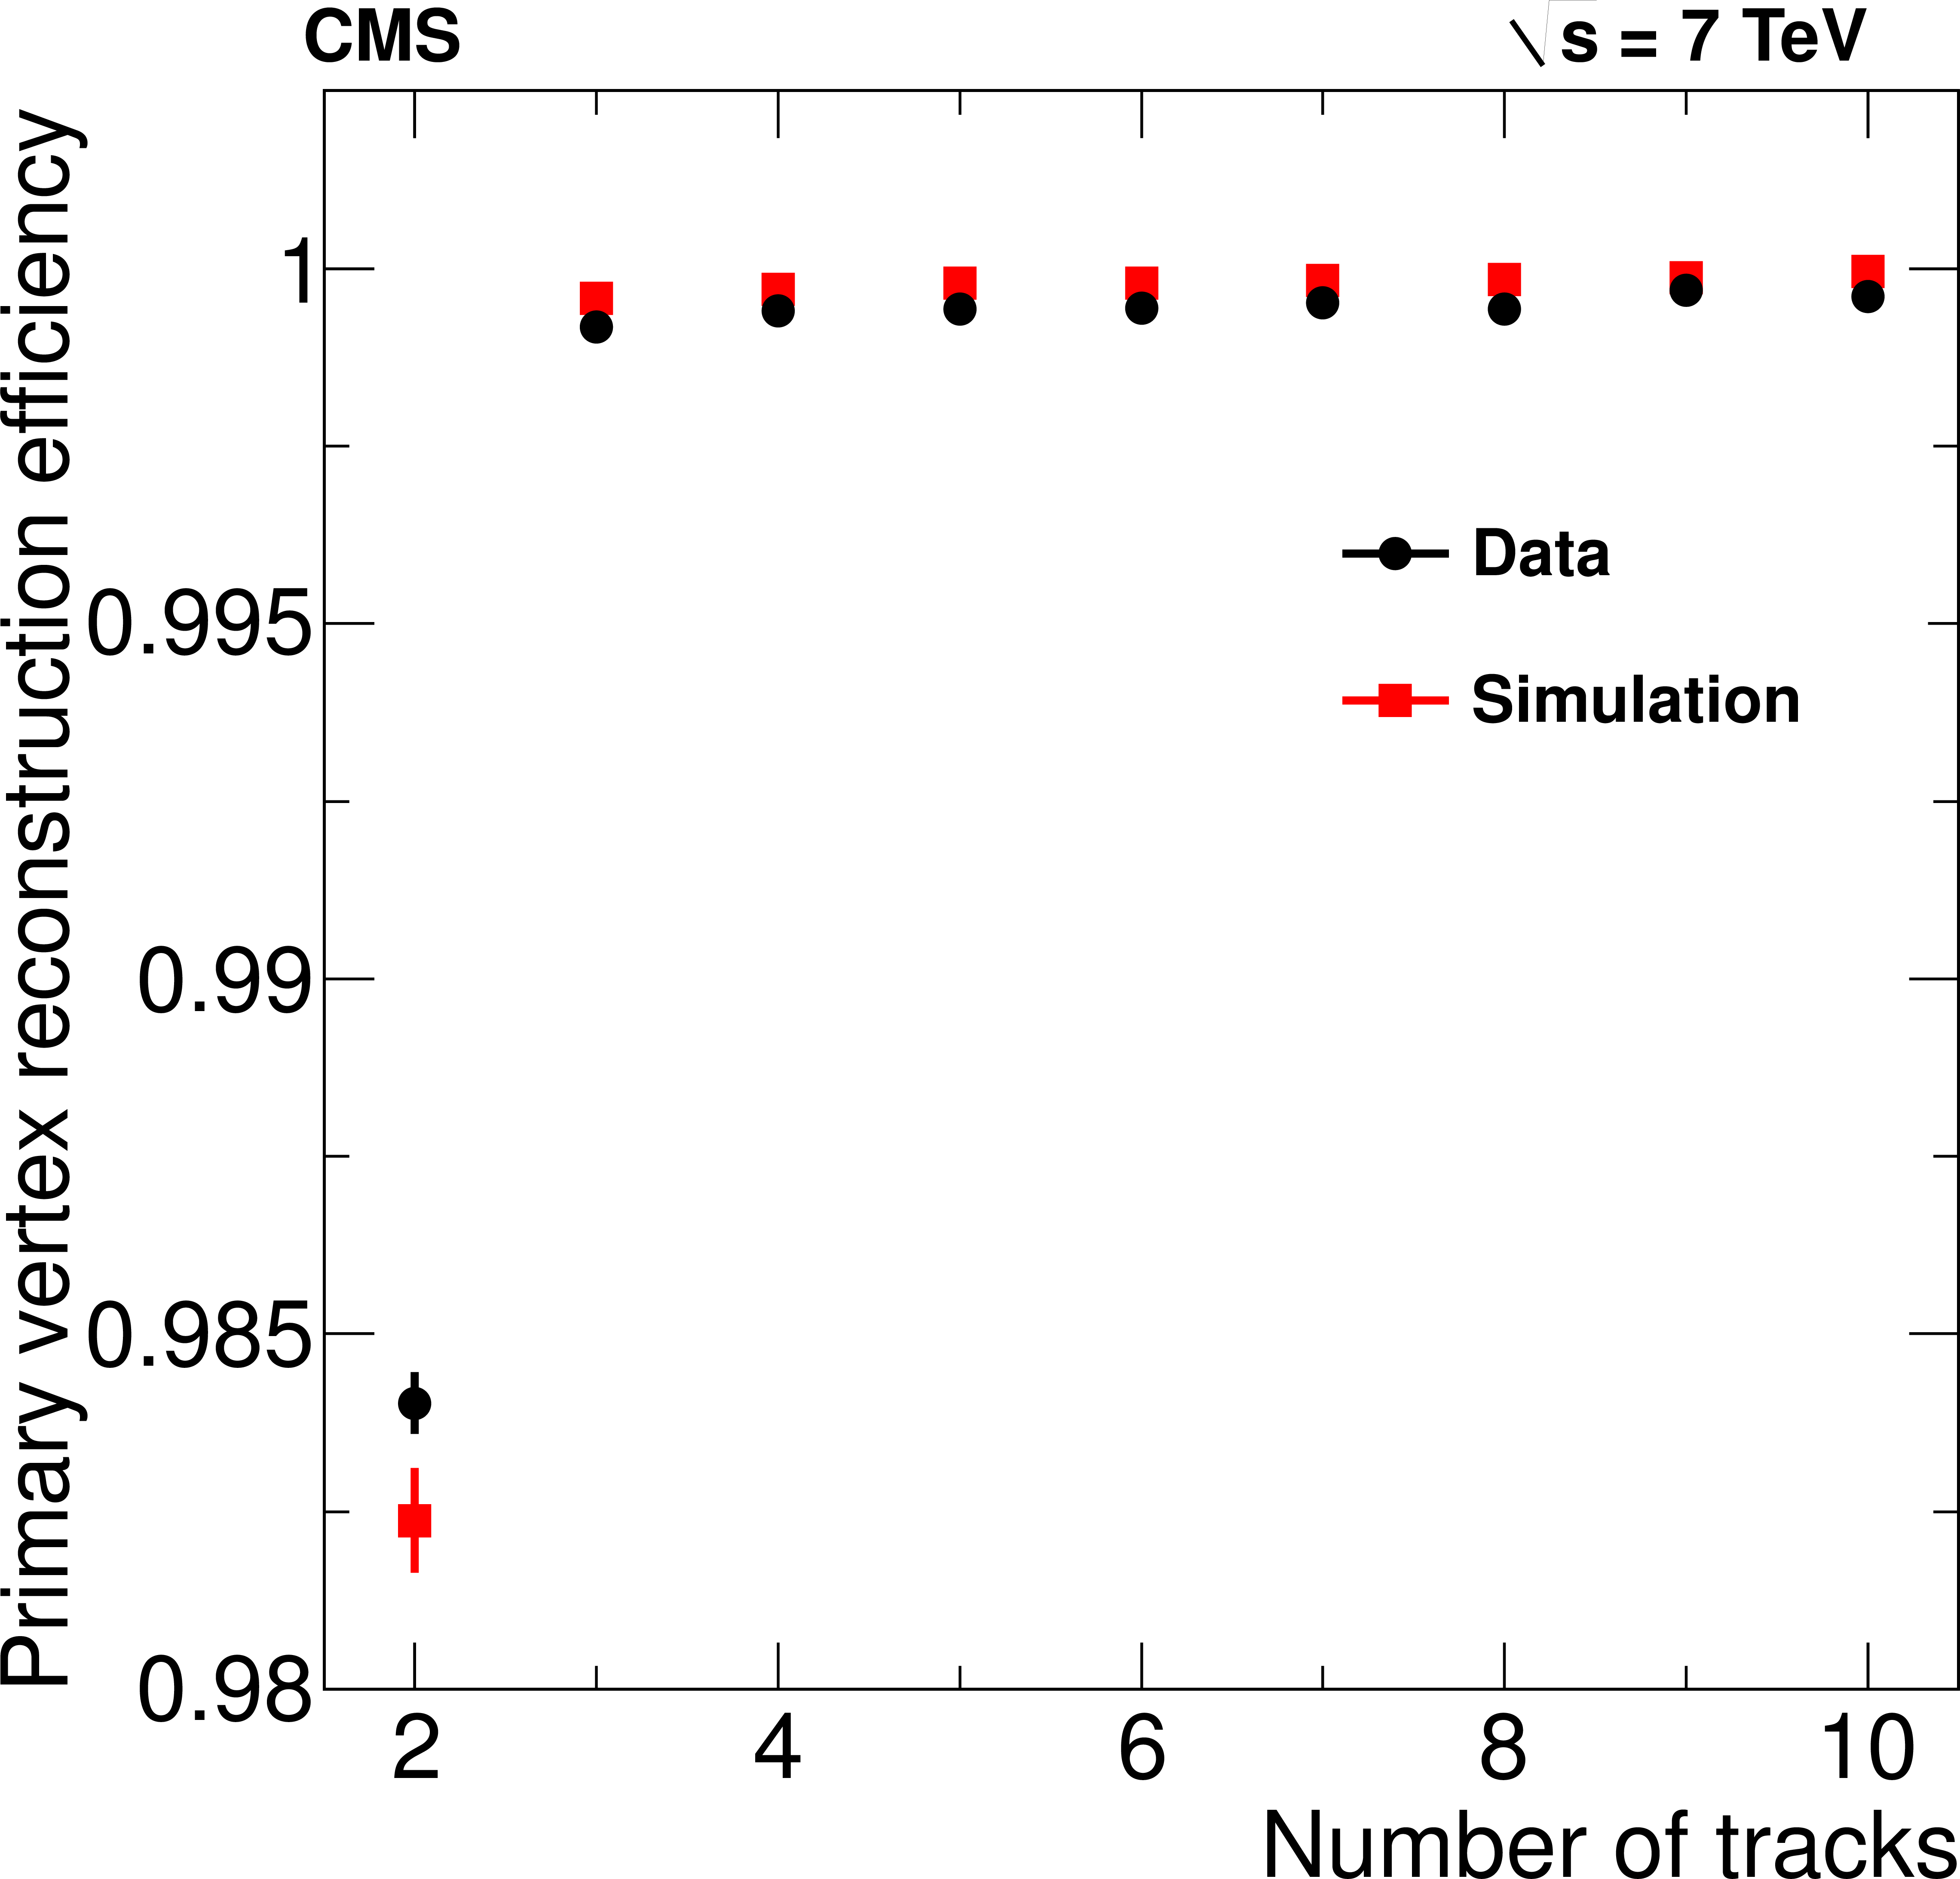
\includegraphics[width=0.32\columnwidth]{figures_chapter4/vertex_efficiency}
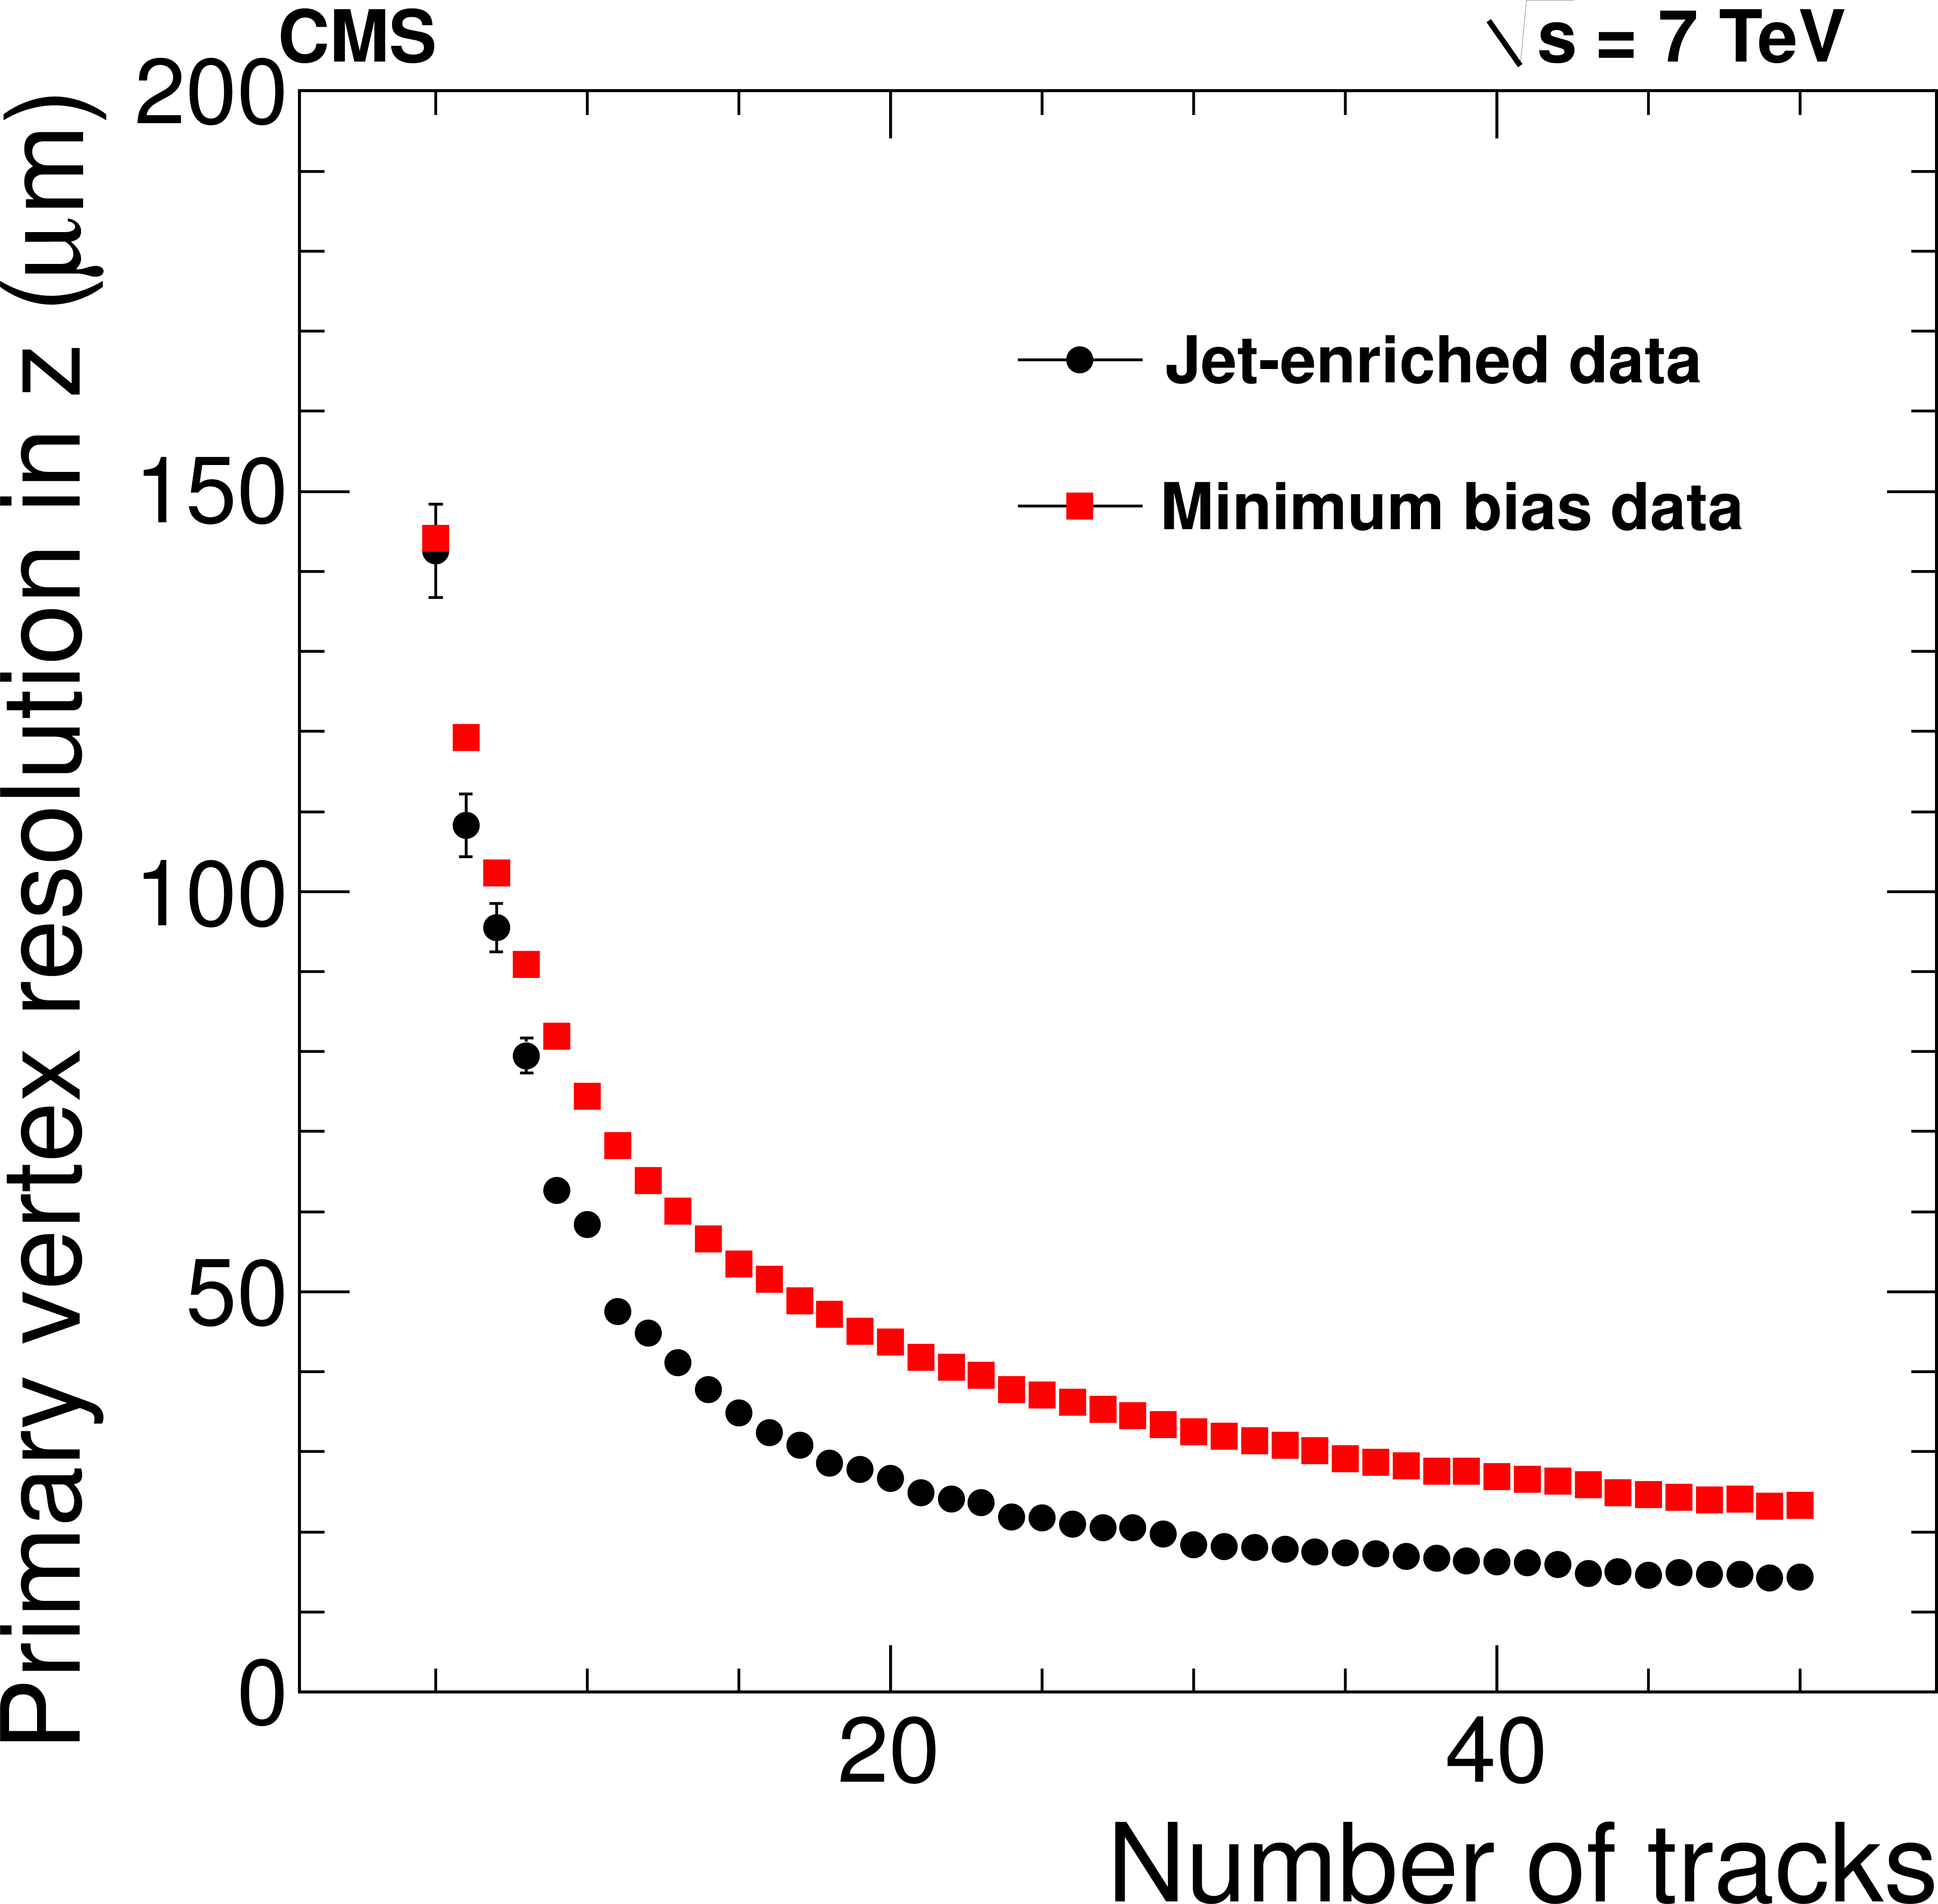
\includegraphics[width=0.32\columnwidth]{figures_chapter4/vertex_resolution}
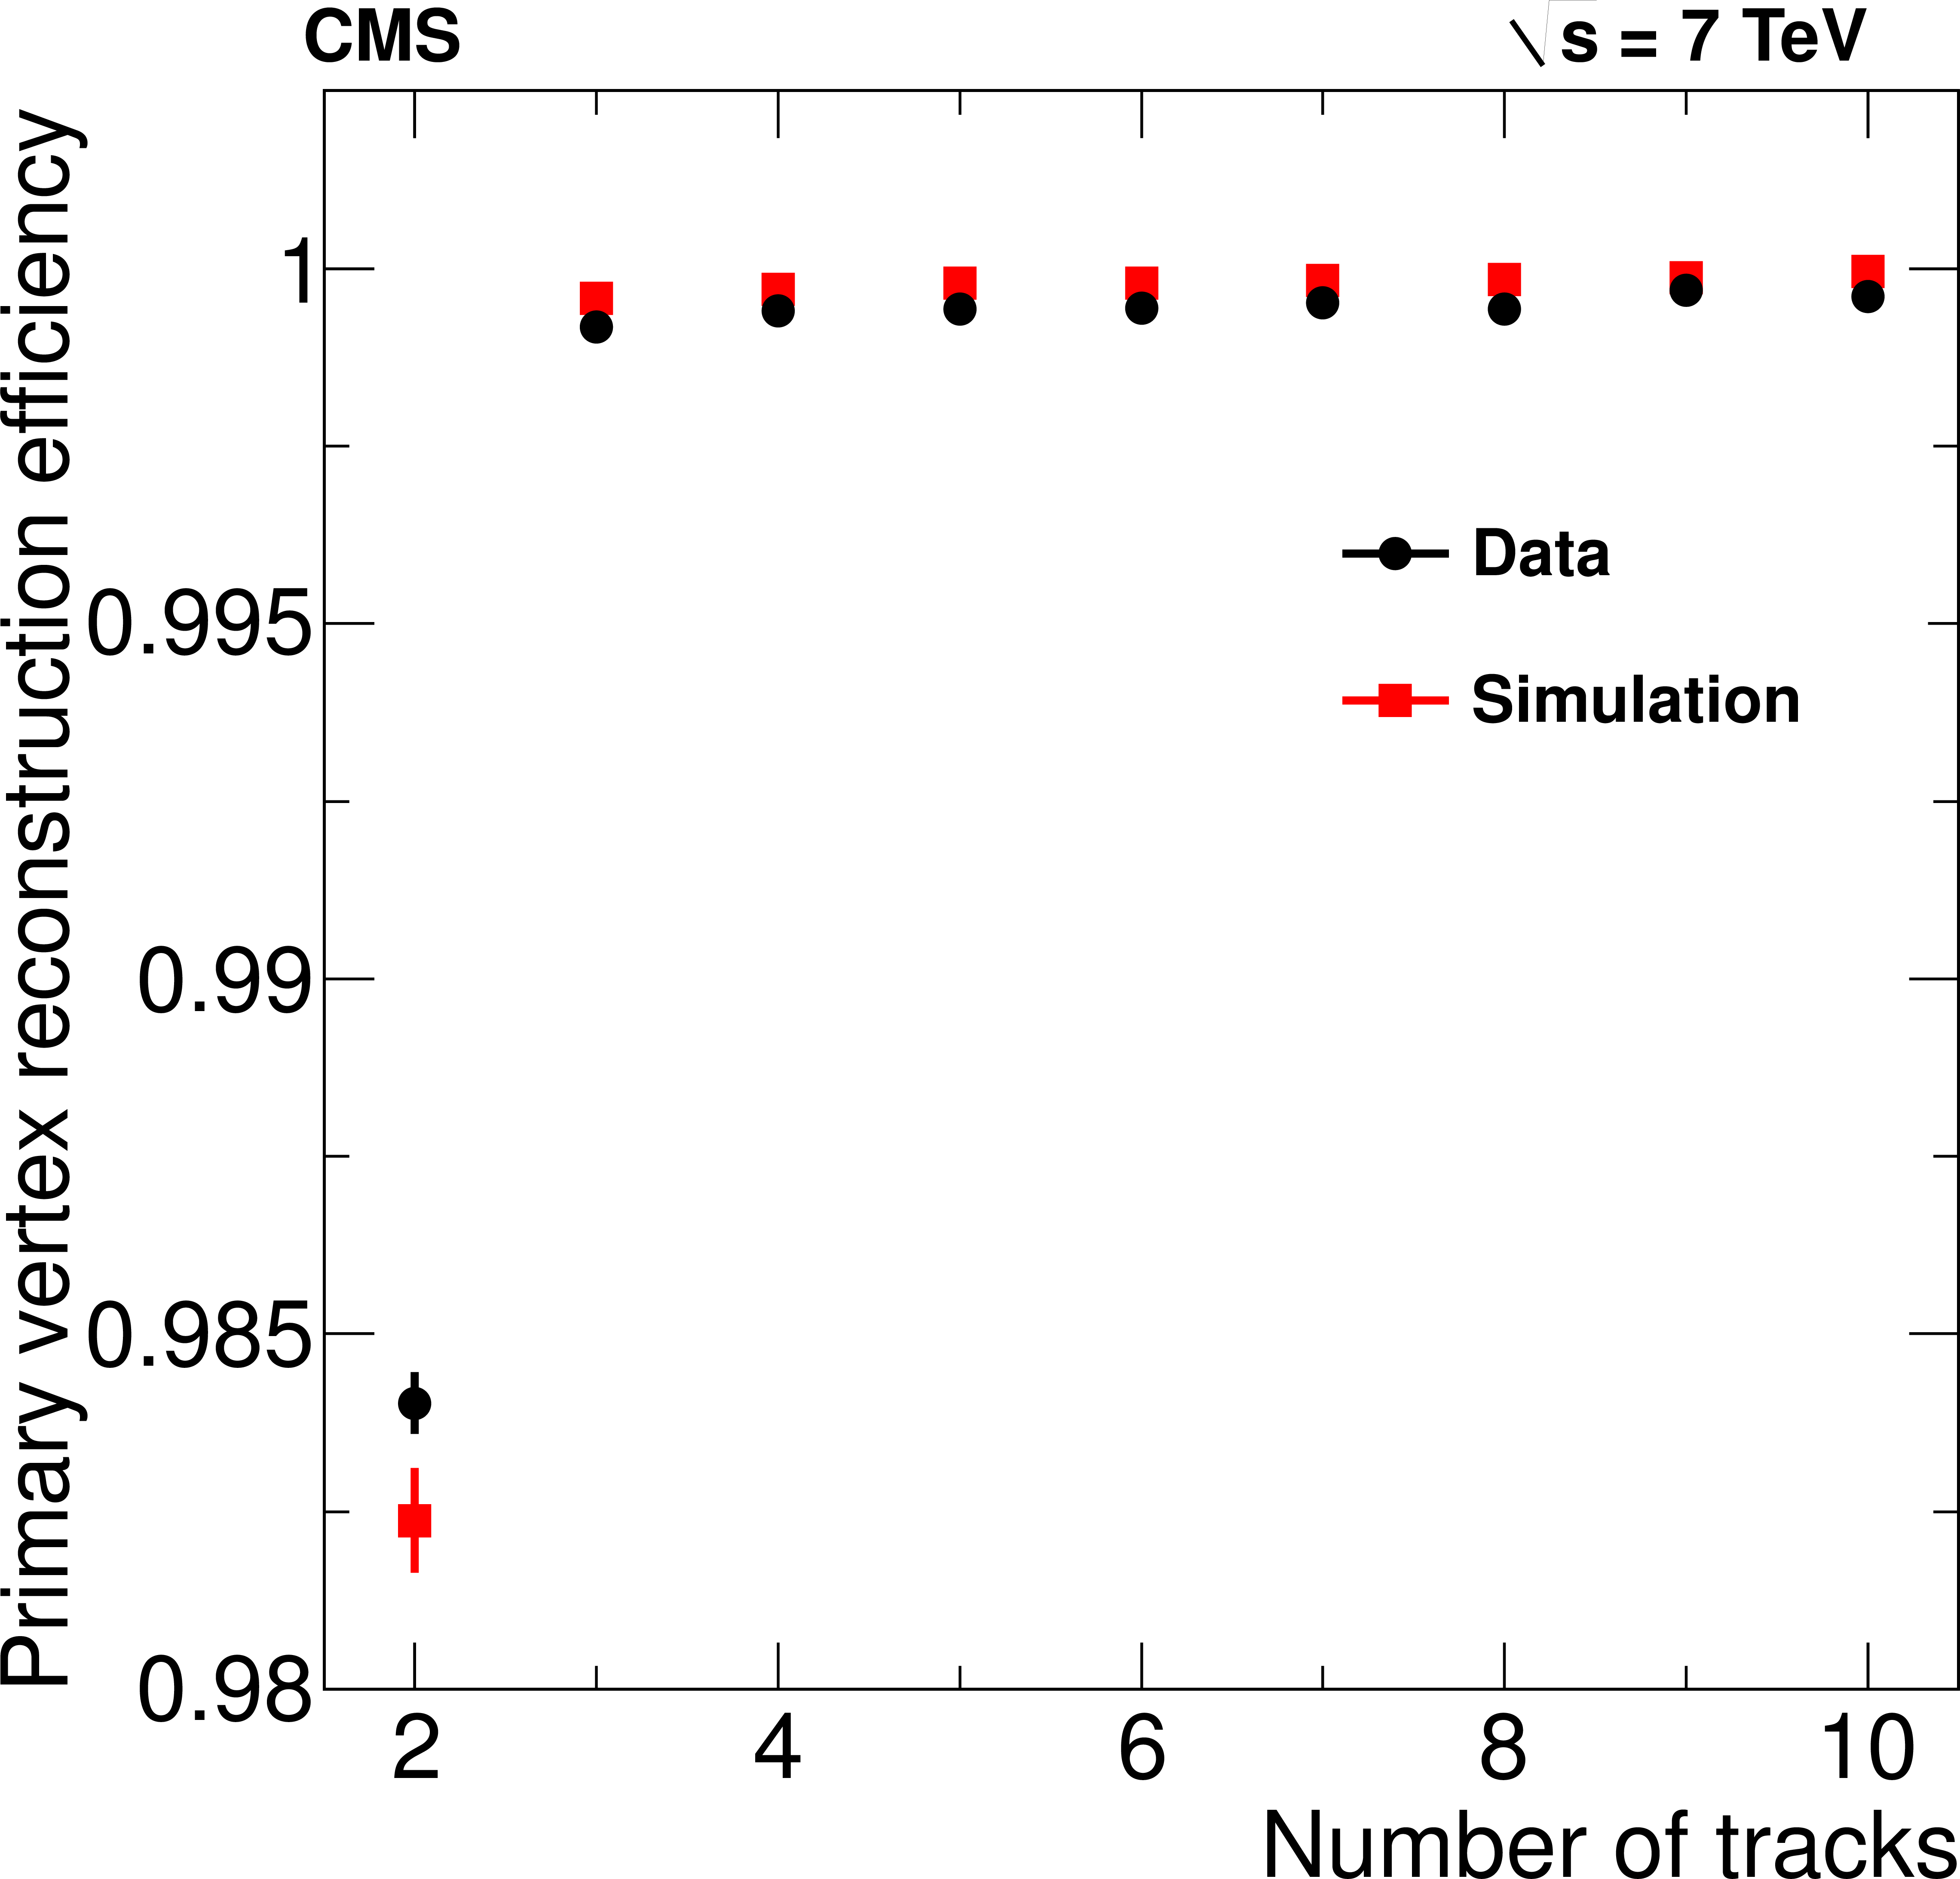
\includegraphics[width=0.32\columnwidth]{figures_chapter4/vertex_efficiency}
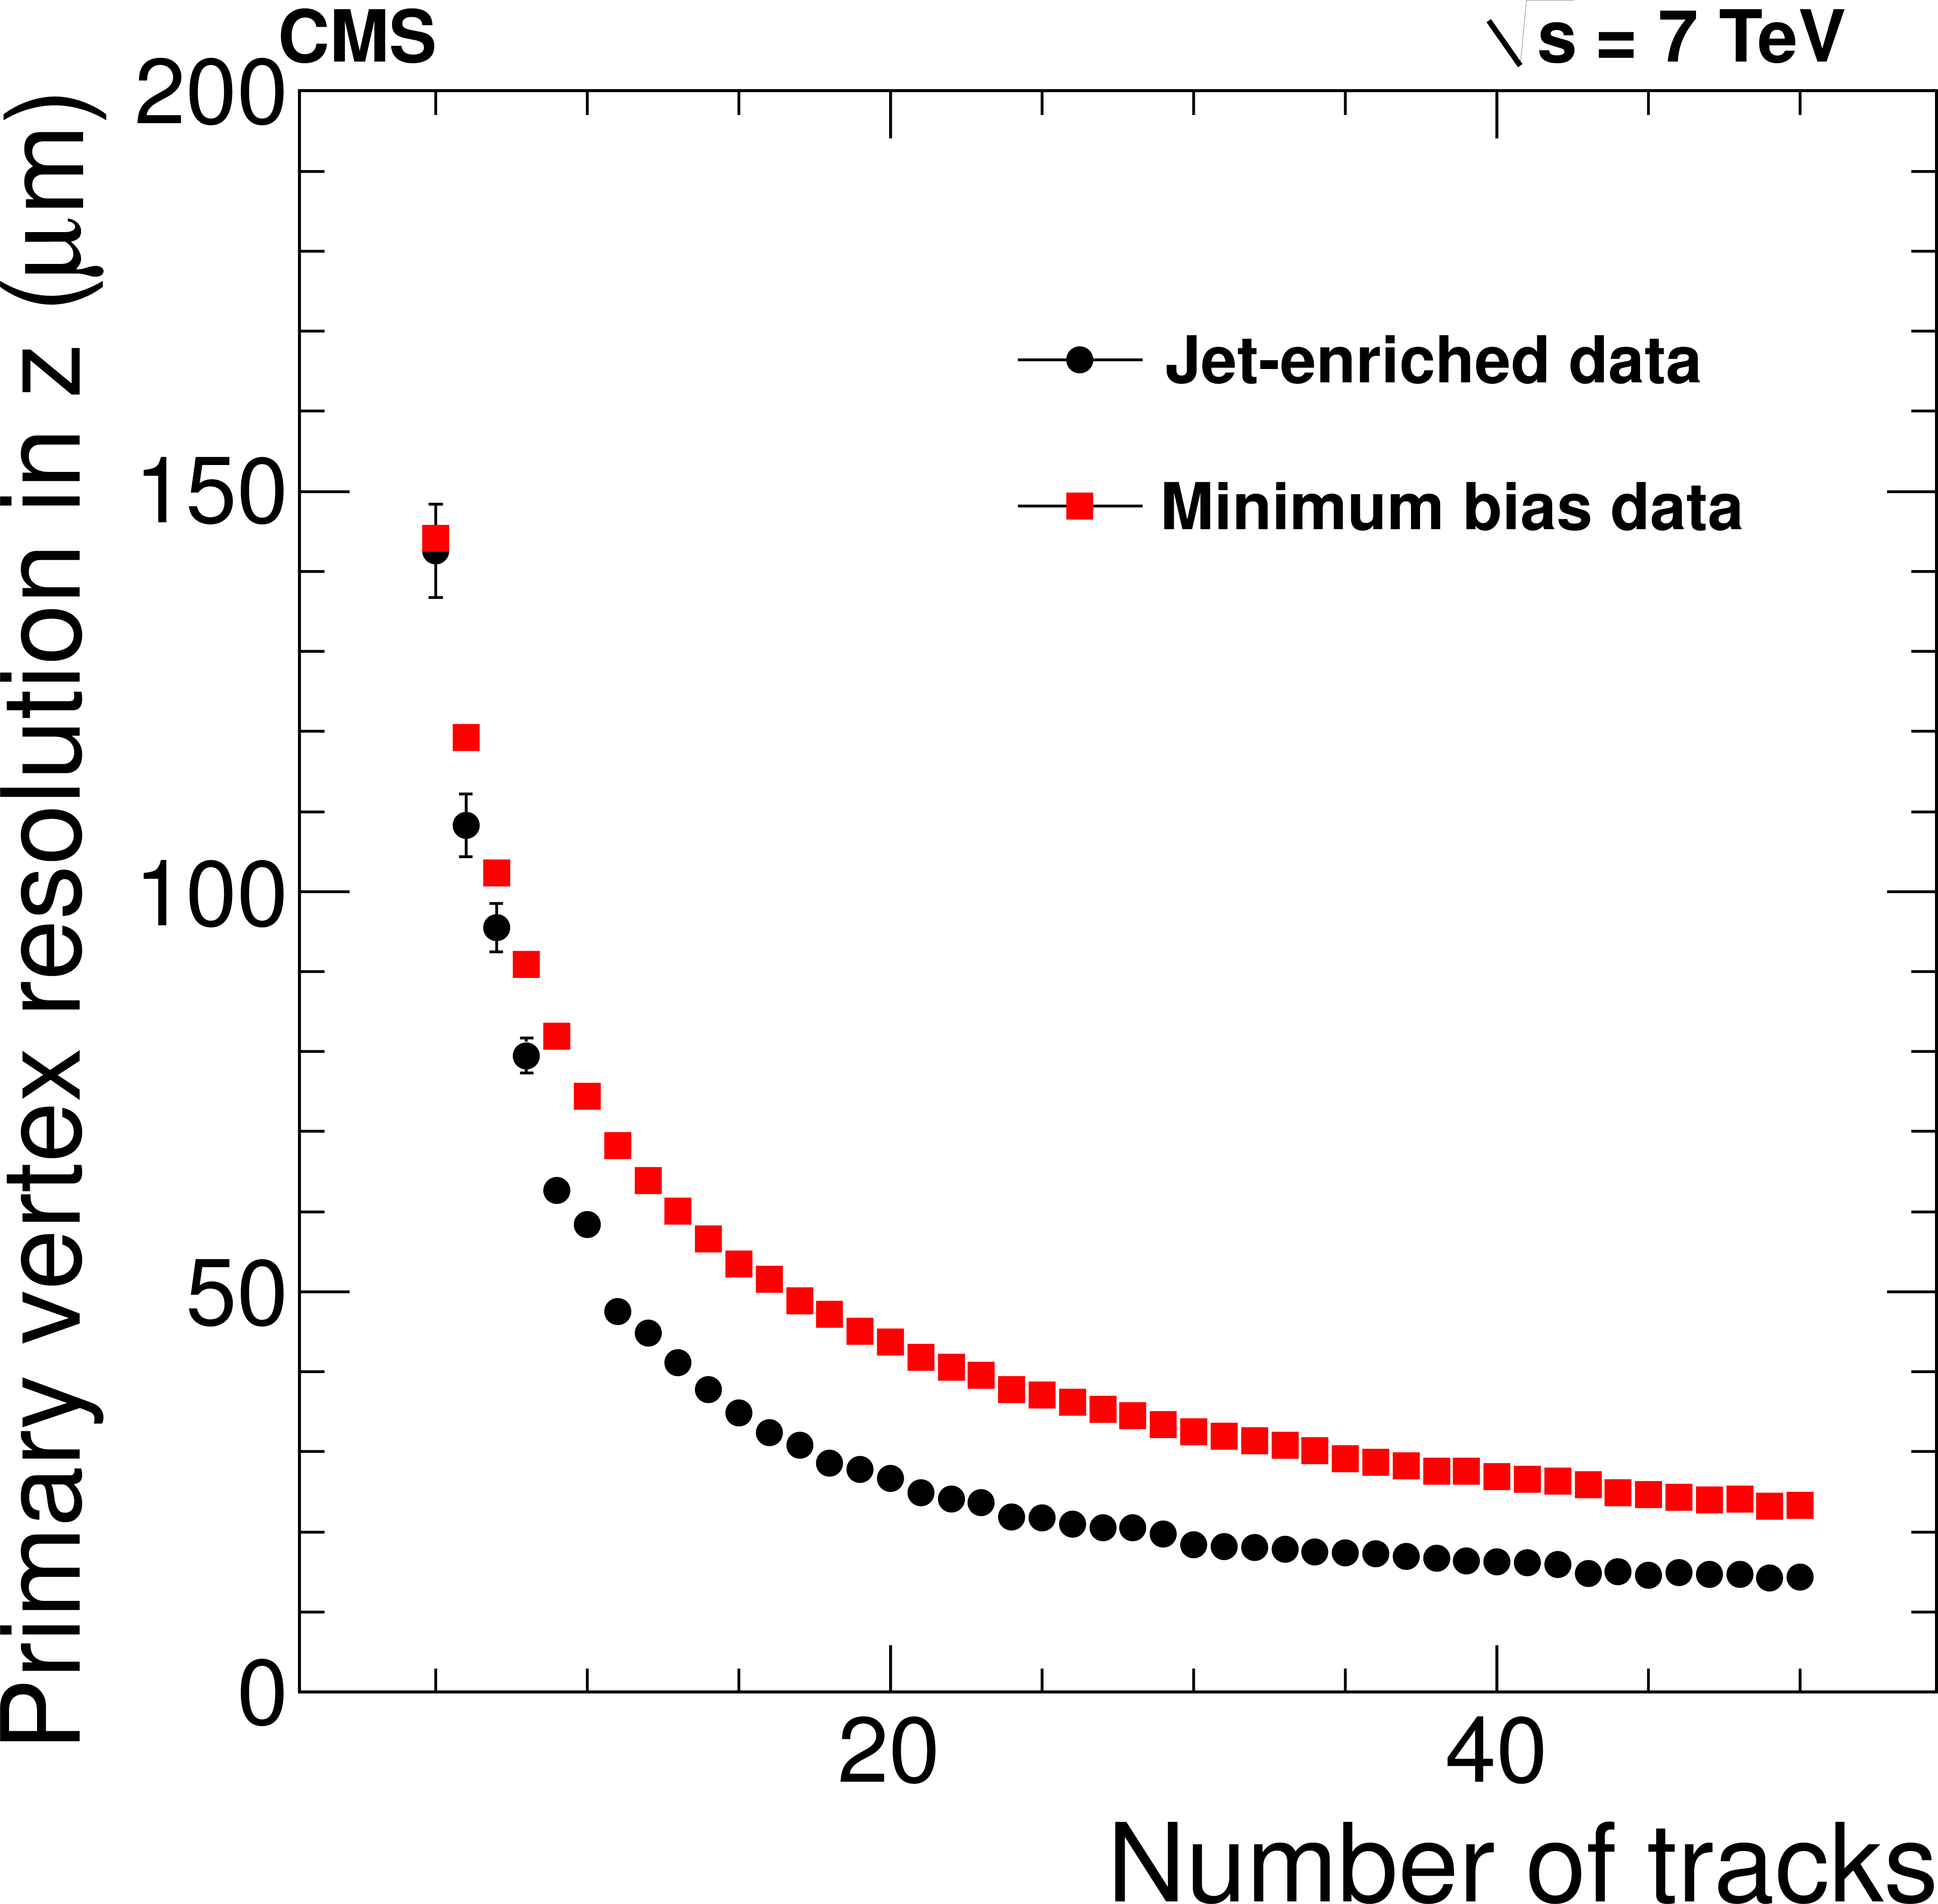
\includegraphics[width=0.32\columnwidth]{figures_chapter4/vertex_resolution}
\caption{Distribution of shower shape $\sigma_{\eta \eta}$, H/E, and $\Delta \eta$ for data at $\sqrt{s}=13~\TeV$ taken during $2015$ data taking period for the barrel (left) and endcap (right). Simulated $W \rightarrow e \nu$ signal process normalized to the number of observed data evens is shown for comparison. The events satisfy all other selection requirements (including the isolation requirement to be discussed in chapter $4$) are satisfied except that on the shown variable.}
\label{fig:ele_id}
\end{figure}

In the ECAL barrel region the energy is collected in a small $\eta$ window and an extended window in $\phi$.  An array of $5\times1$ crystals in $\eta-\phi$ are formed around a seed crystal with transverse energy $E_{T}>1~\GeV$. The arrays are extended in both $\phi$ directions centered at the seed crystals up to $\Delta \phi$ of radius of $0.3$. The arrays withe $E_{T}>0.1~\GeV$ are grouped to form a supercluster. In the ECAL endcap the supercluster is seeded by a $5\times5$ cluster in $\eta-\phi$ that is centered at the seed crystal. The supercluster energy corresponds to the sum of the energies of its clusters. 

Inner tracker seeds compatible with a reconstructed supercluster are searched in the pixel tracker (also in TEC to improve the efficiency). Electrons that suffer small amount of bremsstrahlung radiation loss can be identified by extrapolating a standard reconstructed track to the ECAL and passing close to an ECAL cluster. A poor $\chi^2$ or few associated hits in the reconstructed tracks may come from an electron that suffered a significant bremsstrahlung energy loss. A modified version of the Kalman filter is used to perform the final fit of the parameters as the Kalman filter is optimal for Gaussian uncertainties whereas the bremsstrahlung energy loss is modeled by Bethe-Heitler.  A gaussian approximation to the Bethe-Heitler model is crude and therefore a Gaussian-Sum filter (GSF)~\cite{Adam:815410} method is employed that approximates the Bethe-Heitler energy loss by a sum of Gaussian functions. Electron momentum is derived from a weighted mean of the inner tracker measurements and the supercluster energy. 

There are few sources of electron backgrounds. An overlapping charged and neutral pions inside a hadronic jet or a charged pion showering early in the ECAL can be miss-identified as an electrons. Figure~\ref{fig:ele_id} shows the distributions of few of the electron identification variables used for reduction of these background processes:
 
\begin{description}
\item[$\bullet$]  $\sigma_{\eta\eta}$ is the energy weighted $\eta$ width of the cluster. As can be seen it is small for genuine electrons.  
\item[$\bullet$]  H/E is the ratio of the energy deposited in the HCAL to the electromagnetic energy near the seed cluster. .
\item[$\bullet$] $\Delta \eta$ and $\Delta \phi$ are the separations between the supercluster and track directions evaluated at the primary vertex in the $\eta$ and $\phi$ directions respectively.  
\end{description}

The conversion of a photon into an electron-positron pair is another source of background. Electron candidates with missing hits in the innermost layers of the inner tracker indicate a photon conversion. An identification of a vertex with a pair of tracks with no hits in the tracker layers between the vertex and the interaction point is also used to further suppress this background.


\section{Jet Reconstruction}

Quarks and gluons produced at the LHC fragment and hadronize nearly immediately to a collimated spray of hadrons known as jets. Jets may originate from $2 \rightarrow 2$ scattering of the partons inside the colliding protons, decay of heavy objects such as a top quark or a Higgs boson, and emission of gluons off some other partons in the event. Measuring the jet energy and direction provides information of the original parton. A detailed review of jet finding algorithms, set of rules for grouping hadrons into jets, at hadron colliders can be found in~\cite{Salam:2009jx}. So called sequential recombination jet algorithms are used at CMS as implemented in the FastJet package~\cite{Cacciari:2011ma}.  The usual approach of these algorithms is to introduce two distance measures $d_{ij}$ and $d_{iB}$ defined as:

\begin{eqnarray} \label{eq:jet_find}
d_{ij} = min(p_{ti}^{2p},p_{tj}^{2p})\frac{\Delta_{ij}^2}{R^2}, \\
d_{iB} = p_{ti}^{2p},
\end{eqnarray}

where $\Delta_{ij}^2 = (y_{i}-y_{j})^2 + (\phi_{i} -\phi_{j})^2$ and $k_{ti}$, $y_{i}$, and $\phi_{i}$ are the transverse momentum, rapidity, and azimuth of object $i$ in the event . $R$ is the distance parameter and $p$ is the power of the energy scale. From the above definitions it is seen that $d_{ij}$ and $d_{iB}$ are invariant under a boost along the beam direction. The algorithm proceeds to identify the smallest distance measures in the events. If $d_{ij}$ is the smallest for a given pair of objects, then the two objects are combined into a single object by adding the momenta of the $i$ and $j$ objects. If $d_{iB}$ is the smallest distance then the object $i$ is denoted as a jet and removed from further consideration in the algorithm. The algorithm continues until there are no objects remaining in the event. The anti-$k_{t}$ algorithm~\cite{Cacciari:2008gp} with $p=-1$ is used for the results shown here. A distance parameter of $R=0.5$ or $R=0.4$ is used. The anti-${k_{t}}$ algorithm grows outward from hard "seeds" resulting in a cone-like jets in $\eta-\phi$. The resulting jet boundaries are resilient with respect to soft radiation while the algorithm is infra-red and collinear safe.  


\subsection{Jet Energy Scale Corrections}

Jet energy needs to be calibrated to obtain more accurate estimate of the original parton energy. Corrections are needed to account for the additional energy due to pileup, non-uniformities in the detector response, and detector noise. The effect of additional energy due to pileup and detector noise is corrected on per-jet basis for each event using the median energy density $\rho$ and the jet area~\cite{Cacciari:2007fd}. Pseudorapidity and jet transverse momentum dependent corrections are derived in simulated events with and without pileup overlay. "Zero-bias" triggered events (from randomly selected non-empty LHC bunch crossings) are used to correct for the residual differences between data and detector simulation.  The average jet energy scale is calibrated using the Monte Carlo truth in simulation~\cite{1748-0221-6-11-P11002,Khachatryan:2016kdb}. Corrections are then applied to to account for residual differences  between the detector simulation and data using the transverse momentum balancing in di-jet events, $\gamma$-jet, and $Z$-jet events. The di-jet $p_{T}$ balancing method is used to correct the relative scale using the barrel region $|\eta|<1.3$ as a reference. The absolute scale is corrected using $\gamma$-jet and $Z$-jet events exploiting the excellent $p_{T}$ resolution of photons and leptons. 

\begin{figure}[h]
\centering
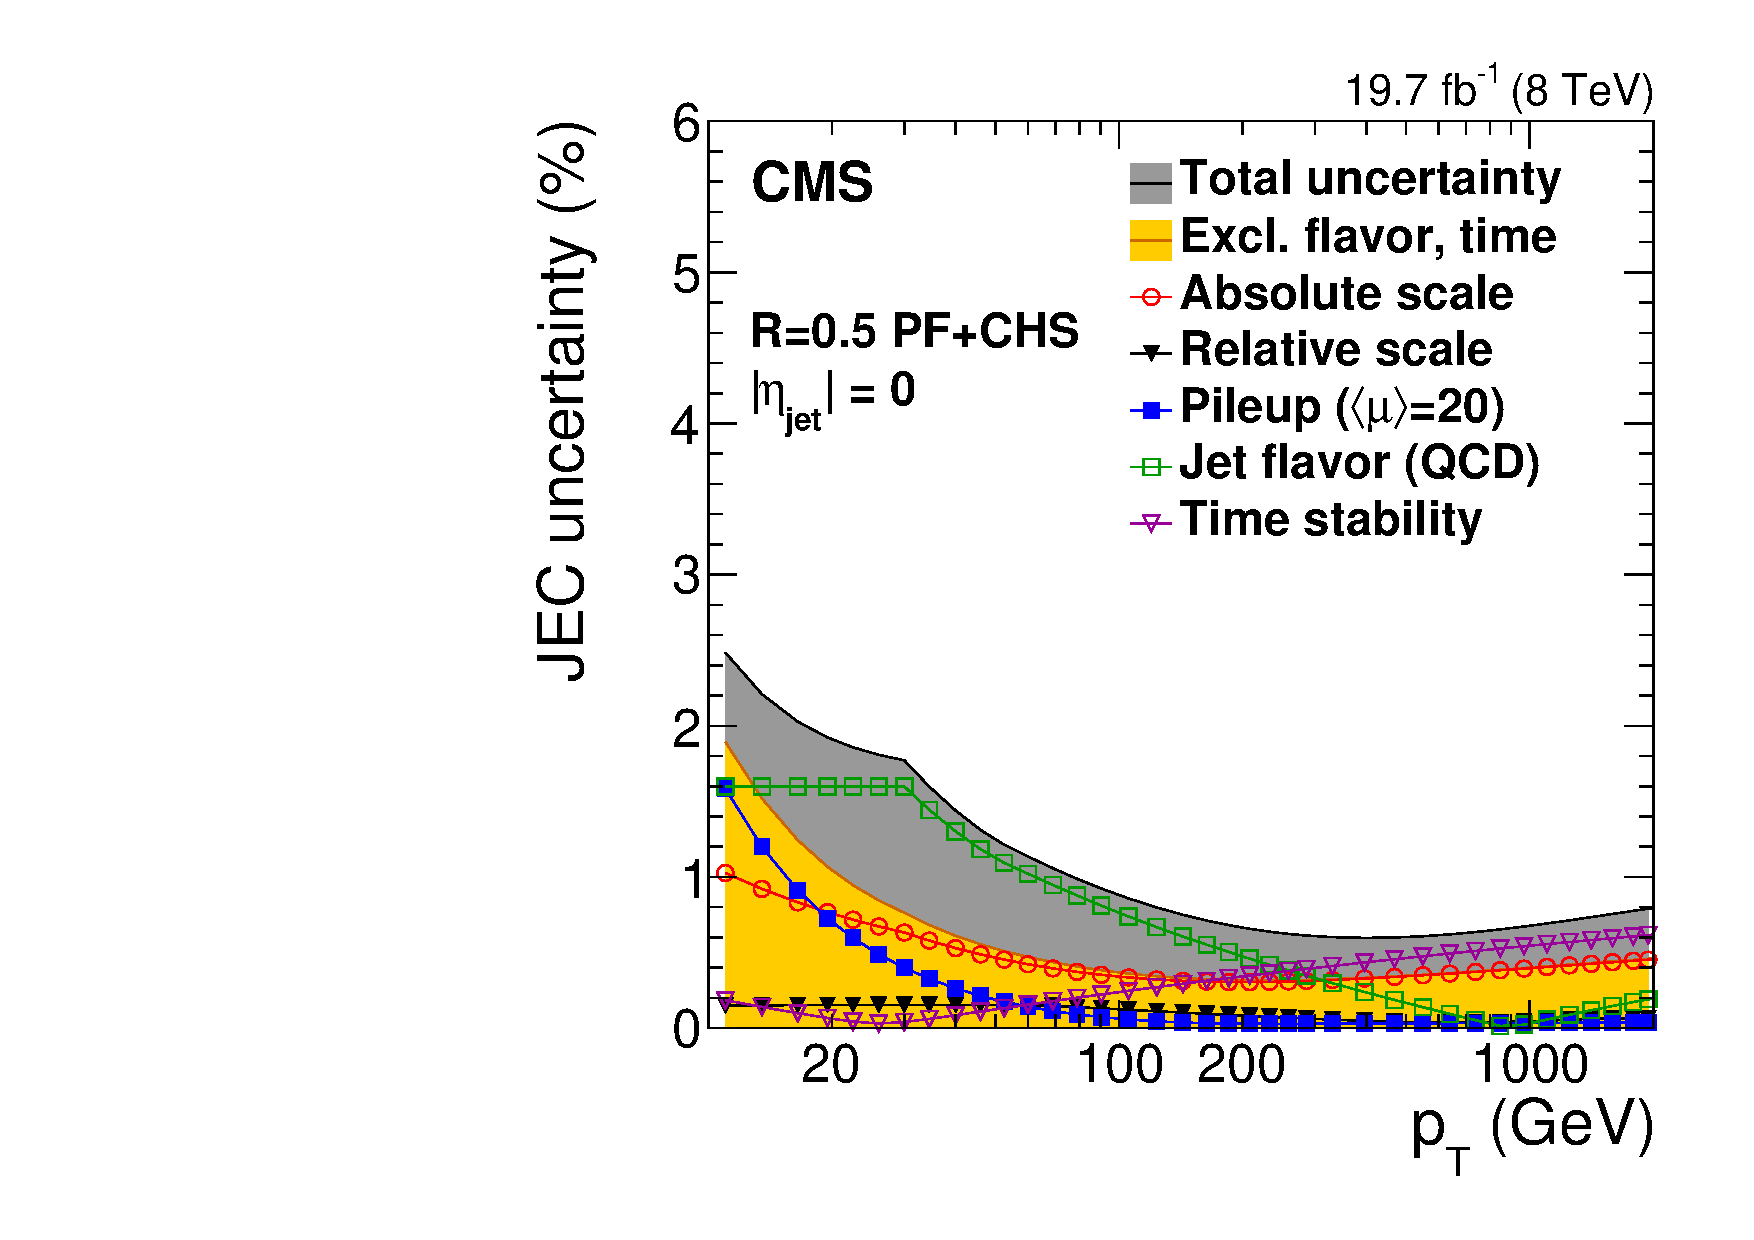
\includegraphics[width=0.49\columnwidth]{figures_chapter4/jec_unc}
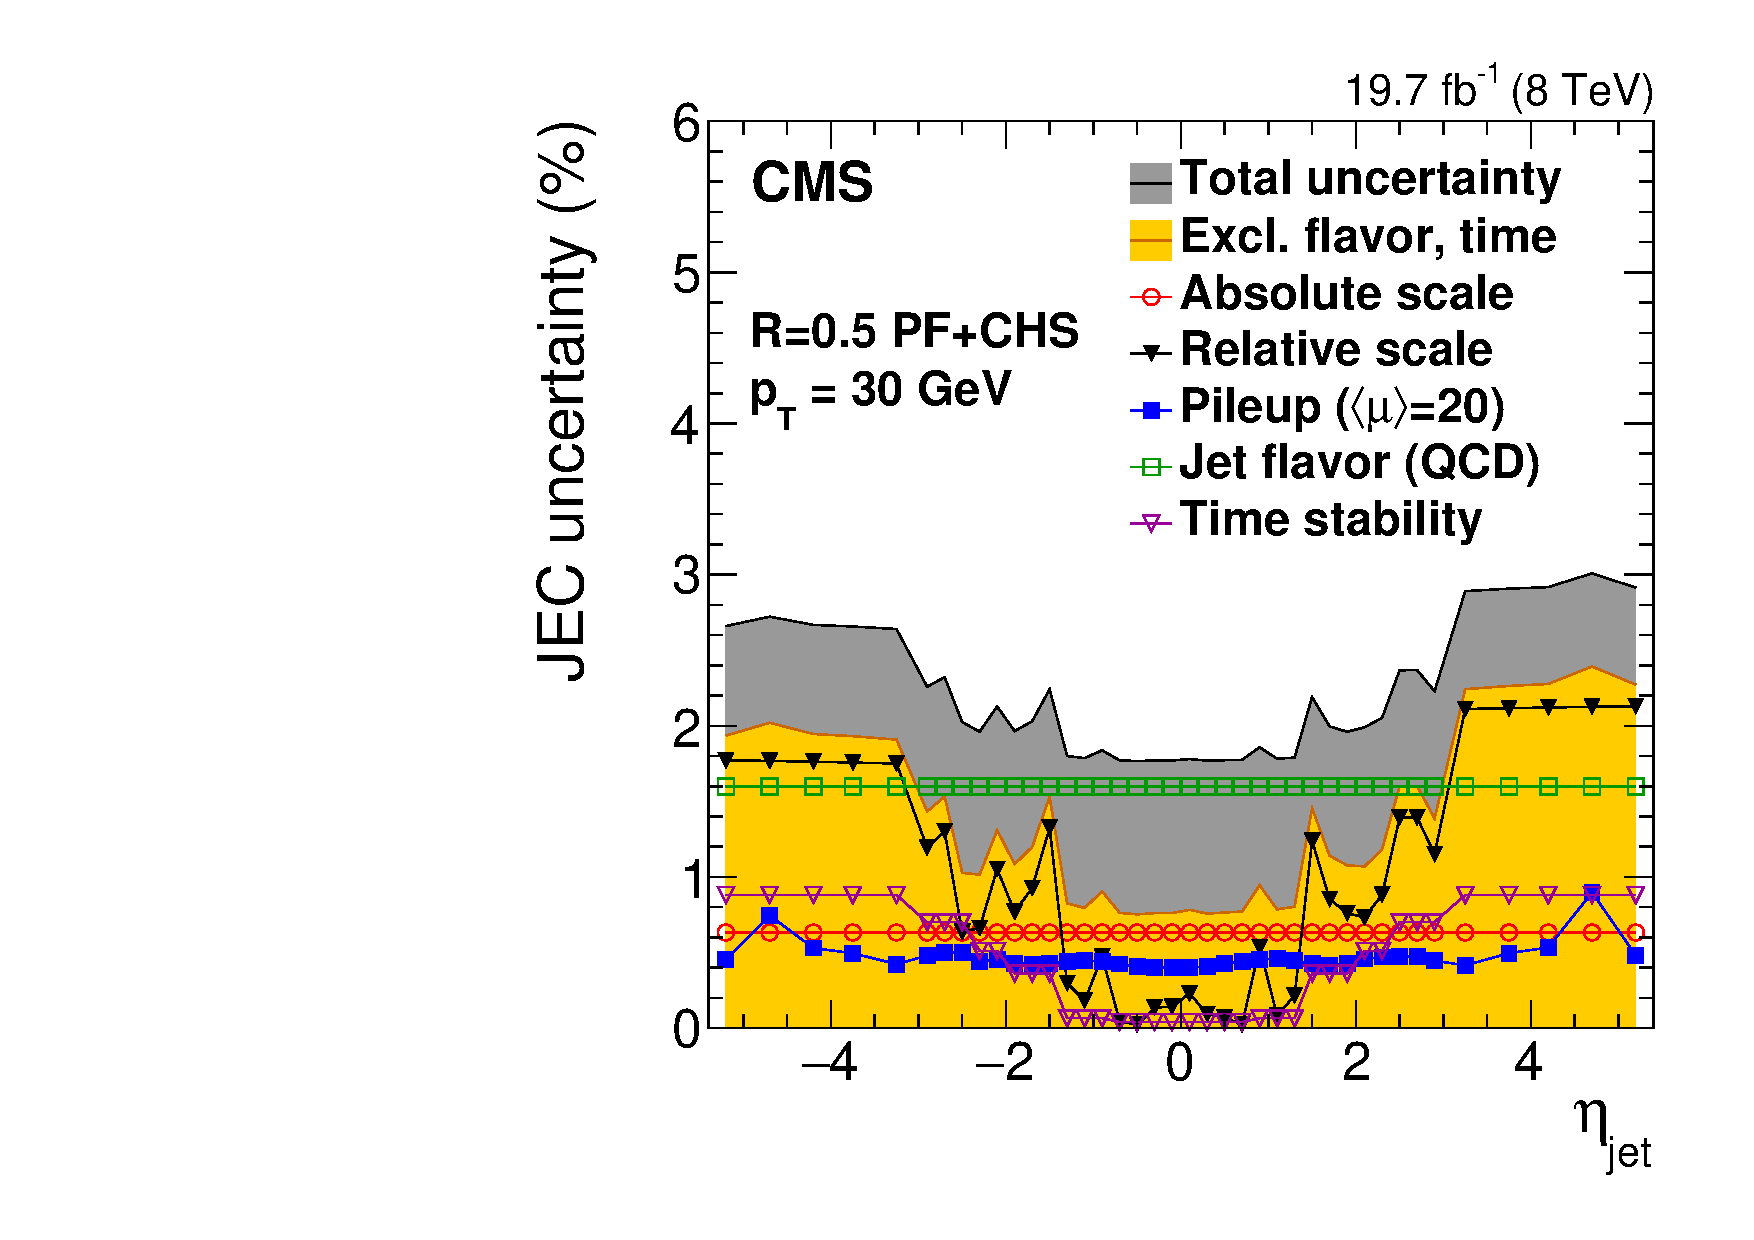
\includegraphics[width=0.49\columnwidth]{figures_chapter4/jec_unc2}
\caption{Summary of jet energy scale systematics as a function of jet $p_{T}$ for $|\eta|=0$ (left) and of jet $\eta$ for $p_{T}=30~\GeV$ at $\sqrt{s}=8~\TeV$ data taking period. The markers show the single effect of different sources and the gray dark band shows the cumulative total uncertainty. The total uncertainty, when excluding the effects of time dependence and flavor, is also shown in yellow light~\cite{Khachatryan:2016kdb}.}
\label{fig:jet_unc}
\end{figure}

Figure~\ref{fig:jet_unc} shows the summary of jet energy scale uncertainty as a function of jet $p_{T}$ and $\eta$ at $\sqrt{s}=8~\TeV$ data taking period. Jets selected for majority of the physics results are required to have a transverse momentum greater than $30~\GeV$ (the $p_{T}$ requirement is lower for jets originating from b quarks) with $|\eta|<4.7$.  The uncertainties on the jet energy scale are below $3\%$ across the phase space considered by most analyses and below $1\%$ in the barrel region when excluding the uncertainties due to jet flavor differences at different stages of the corrections.

\subsection{b-jet identification}



\section{Particle Flow}

CMS uses so called particle flow (PF) approach to calorimetry~\cite{CMS-PAS-PFT-09-001,CMS-PAS-PFT-10-001,CMS-PAS-PFT-10-002}.  The basic idea of the PF approach is to combine the information from all the sub-detectors in order to reconstruct all the particles in the event using the best measurements possible. This is especially useful for jet energy measurements as roughly $62\%$ of the jet energy is carried by charged particles (mainly hadrons), around $27\%$ by photons, about $10\%$ by long lived neutral hadrons, and around $1.5\%$ by neutrinos~\cite{Thomson200925}. Thus, one can exploit the superior momentum (energy) resolution of the inner tracker (ECAL) to obtain the most accurate measurements for the charged hadrons (photons) inside the jet. In addition, the high granularity ECAL makes it possible to separate the photons from the charged particle energy deposits. 

 The basic elements of the PF algorithm are tracks in the inner tracker, muon segments in the muon system, and energy clusters from the calorimeters. The calorimeter clustering allows to separate the neutral particles from the energy deposits of charged hadrons as well as to reconstruct and identify the electrons and the corresponding Bremsstrahlung photons. The clustering starts from the cluster seed defined as a local energy maxima. The clusters are then grown from the seeds by including neighboring cells with an energy in excess of a defined threshold in the cluster. The threshold is defined to be two standard deviation of the electronic noise of the ECAL ($80~\MeV$ in the barrel and  approximately $300~\MeV$ in the endcap) and $800~\MeV$ in the HCAL. A linking algorithm is required as a given particle will result in several PF elements. This is achieved by defining a distance measure between each pair of PF elements. For example, the ECAL clusters of the bremsstrahlung photons emitted by an electron are linked by extrapolating the tangents of the track at each intersection point of the track and the inner tracking detector layer to the ECAL to form a PF block. It has to be noted that due to high granularity of the CMS detector the linked blocks typically contain only $1-3$ elements. 
 
 The PF candidates are identified from these blocks. The block and the corresponding PF elements are iteratively removed from further consideration once a PF candidate has been identified. A global muon is denoted as a PF muon if a track element is compatible with the global muon. The track is removed from further consideration and the expected energy deposits in the calorimeters are subtracted from the corresponding calorimeter clusters.  The GSF electron tracks are linked to the ECAL clusters using a discriminator against charged pions that utilizes information from the inner tracker and the ECAL. A PF electron is formed from the GSF tracks and the ECAL clusters (including the clusters identified as bremsstrahlung photons) in case of a positive match. The remaining inner tracker tracks are identified as charged hadrons. If the linked calorimeter cluster energy exceeds the tracker momentum (taking the relevant measurement uncertainties into account) the energy excess is identified as a neutral particle. In addition a PF photon is identified if the excess energy is larger than the linked ECAL cluster while the remaining energy is assigned to a neutral hadron. The remaining ECAL (HCAL) clusters that do not have a linked track are denoted as PF photons (PF hadrons).   
 
 The output of the PF algorithm are denoted as particle flow candidates and are classified as electrons, photons, muons, charged hadrons, or neutral hadrons. The particle flow candidates are used for the reconstruction of jets (referred as PF jets) as described in the previous section.  

\section{Hadronic Tau Decays}

The $\tau$ lepton with a mass of $1.777~\GeV$~\cite{Agashe:2014kda} is the only lepton sufficiently heavy to be able to decay to hadrons.  Hadronic tau decays proceed via weak interaction into one or three charged pions or kaons with up to two neutral pions, and one tau neutrino ($\nu_{\tau}$). The $\nu_{\tau}$ escapes the detector resulting in a missing energy in the event. The $\pi_{0}$ meson decays almost exclusively to a pair of photons. Table~\ref{tau_decay} summarizes the most common hadronic tau decays. The mean lifetime of the $\tau$ lepton is $290\times10^{-15}$ s~\cite{Agashe:2014kda} resulting in a significant (compared to the transverse impact parameter and secondary vertex resolution) displacement of the decay vertex from the production vertex for energetic taus. The hadronic tau decays are denoted $\tau_{h}$ henceforth.

\begin{table}[htbp]
\begin{center}
\begin{tabular}{lcc} 
\hline 
Decay Mode & Resonance  & Branching fraction $[\%]$   \\ 
\hline 
$\tau^{\pm} -> h^{\pm} \nu_{\tau}$                             &             & 11.5 \\
$\tau^{\pm} -> h^{\pm} \pi^{0} \nu_{\tau}$                    & $\rho(770)$ & 26.0 \\
$\tau^{\pm} -> h^{\pm} \pi^{0}  \pi^{0} \nu_{\tau}$            & $a_1(1260)$            & 10.8 \\
$\tau^{\pm} -> h^{\pm} h^{\pm} h^{\mp} \nu_{\tau} $            & $a_1(1260)$            & 9.8 \\
$\tau^{\pm} -> h^{\pm} h^{\pm} h^{\mp} \pi^{0} \nu_{\tau} $ &                         & 4.8 \\
Other hadronic modes &                         & 1.8 \\ 
\hline 
All hadronic modes &                         & 64.8 \\ 
\hline 
\end{tabular}
\caption{Approximate branching fractions of hadronic tau decay modes~\cite{Agashe:2014kda}. The intermediate meson resonances are indicated where appropriate. The symbol $h$ represents a charged pion or kaon.
}
\label{tab:tau_decay}
\end{center}
\end{table}

The visible decay products in the $\tau_{h}$ decays result in collimated jets with lower particle multiplicity. The main idea of the $\tau_{h}$ reconstruction algorithm is to reconstruct the individual decay modes listed in Table~\ref{tau_decay}. The hadron-plus-strip (HPS) algorithm~\cite{1748-0221-7-01-P01001} takes advantage of the PF algorithm combining the reconstructed charged hadrons and neutral particles.  The HPS algorithm starts with a PF jet of $p_{T}$ greater than $14~\GeV$ and $|\eta|<2.5$ using the anti-$k_{T}$ algorithm with distance parameter of $R=0.5$. The photons produced in $\pi^{0} \rightarrow \gamma\gamma$ decays are likely to convert to an electron-positron pair within the volume of the inner tracker. This is taken into account by clustering the electrons and photons (with $p_{T}>0.5~\GeV$)  in the jet into strips in the $\eta-\phi$ plane with a window size of $0.05\times0.20$ taking the direction of the bending of the charged trajectories into account. Strips with total $p_{T}$ sum larger than $2.5~\GeV$ are identified as $\pi^{0}$ candidates. 

$\tau_{h}$ candidates are formed by combining the clustered strips with the charged candidate constituents of the jets. The charged particles are required to have a $p_{T}$ greater than $0.5~\GeV$. The distance of closest approach to the charged particle of highest $p_{T}$ in the jet has to be less than $0.4$ cm in the $z$ direction and $0.03$ cm in the transverse plane~\cite{1748-0221-11-01-P01019}. The following decay hypotheses are considered:

\begin{description}
\item[$\bullet$ $h^{\pm}$:] A single charged particle with no $\pi^{0}$ candidates.  
\item[$\bullet$ $h^{\pm} \pi^{0}$:] One charged particle and one strip with a system mass of $0.3<m_{\tau_{h}}<1.3~\GeV$ for $p_{T}<200~\GeV$. The size of the mass window is enlarged for $\tau_{h}$ candidates with high $p_{T}$ to account for the inner tracker momentum resolution degradation. The mass cut utilizes the mass of the intermediate meson resonance in the decay. 
\item[$\bullet$ $h^{\pm} \pi^{0}  \pi^{0}$:] One charged particle combined with two strips. The mass cut requirement is $0.4<m_{\tau_{h}}<1.2~\GeV$ for $p_{T}<200~\GeV$ targeting the intermediate meson resonance decay of $a_{1} (1260)$.  The size of the mass window is enlarged for $\tau_{h}$ candidates with high $p_{T}$.
\item[$\bullet$ $h^{\pm} h^{\pm} h^{\mp}$:] Combination of three charged particles with mass of $0.8<m_{\tau_{h}
}<1.5~\GeV$. The sum of the charges is required to be $1$. The charged tracks are required to originate from the same event vertex ($\Delta z< 4$ mm).
\end{description}

\begin{figure}[h]
\centering
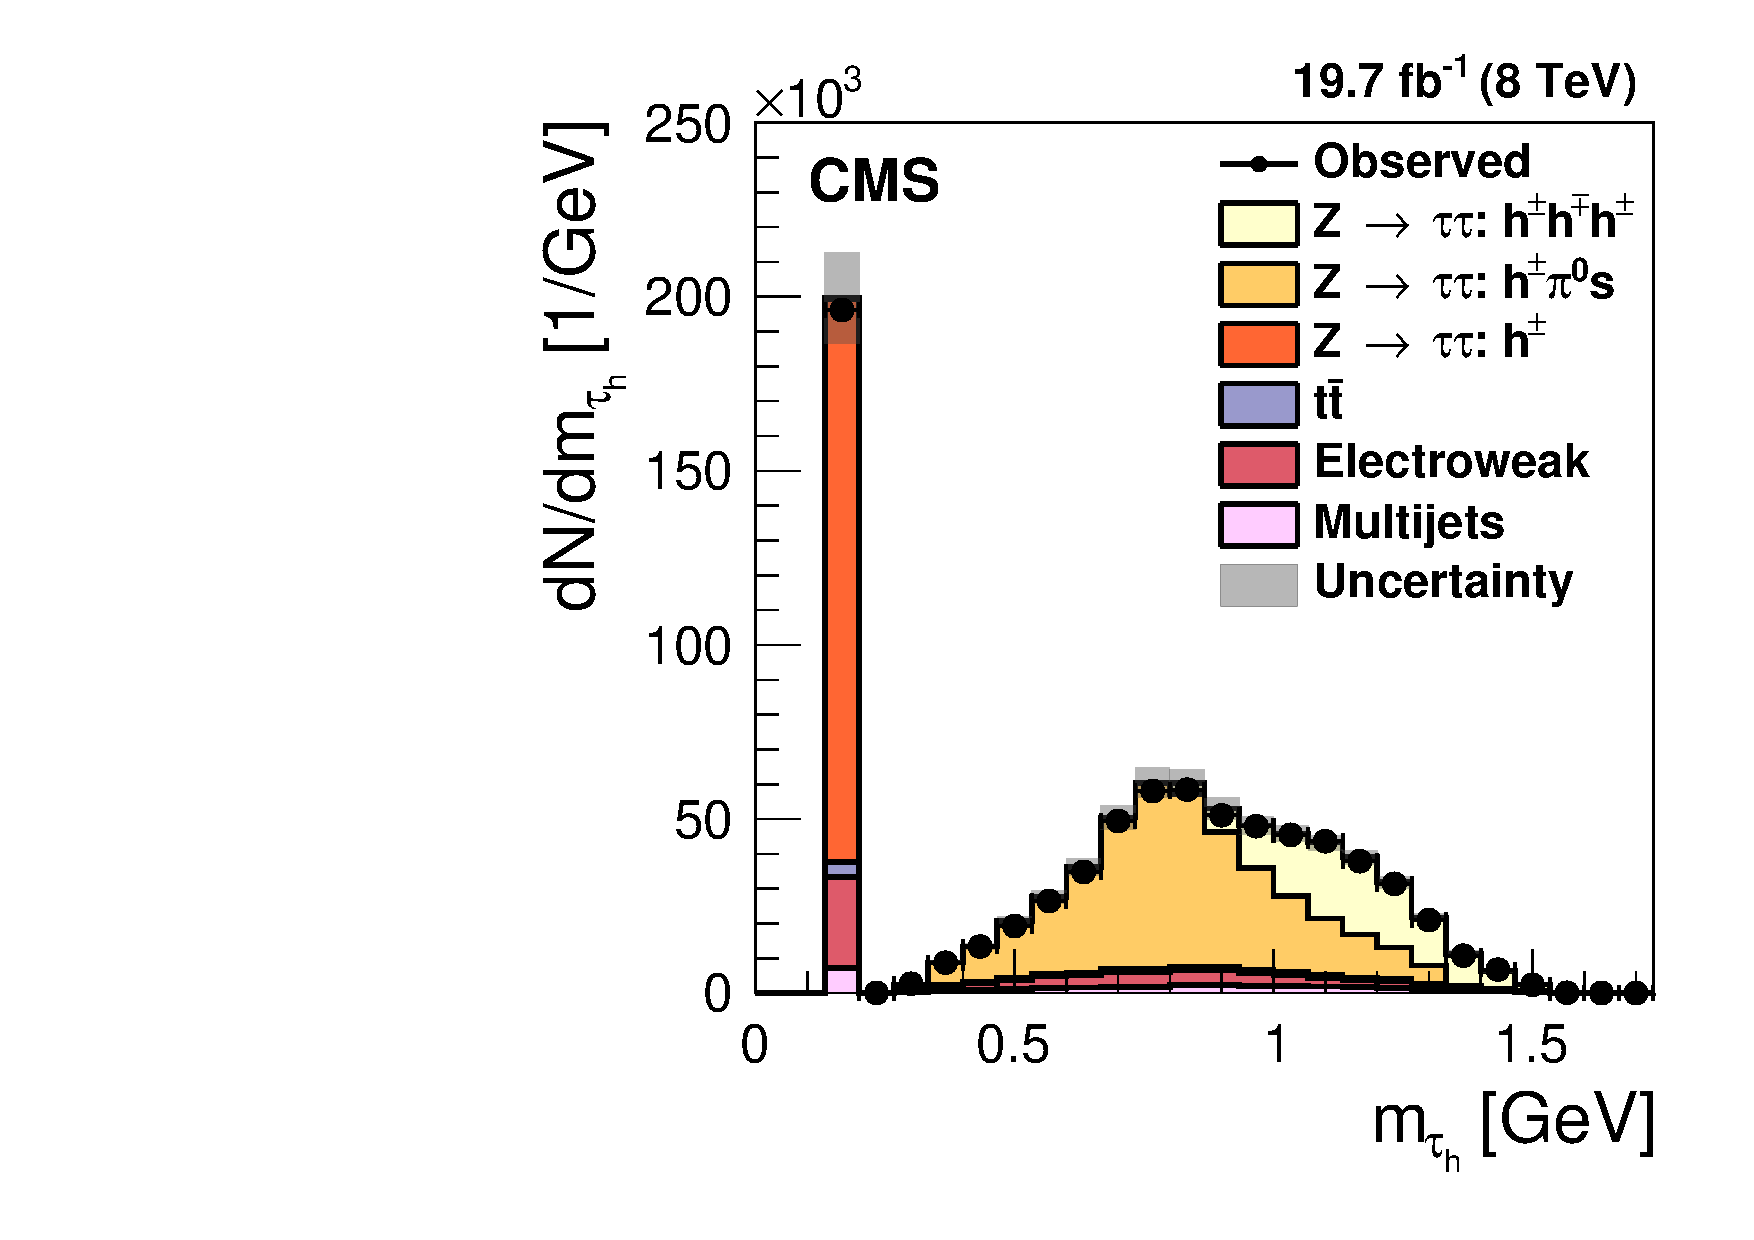
\includegraphics[width=0.80\columnwidth]{figures_chapter4/tau_mass}
\caption{Distribution of the $\tau_{h}$ masses in $Z/\gamma^{*} \rightarrow \tau\tau$ events selected in data during $\sqrt{s}=8~\TeV$ data taking period. Expected predictions from the simulation are also shown. The $Z \rightarrow \tau\tau$ prediction is split into the different expected $\tau_{h}$ decay modes. The electroweak background is mainly due to $W+$jets production~\cite{1748-0221-11-01-P01019}.}
\label{fig:tau_mass}
\end{figure}

An additional requirement is imposed on the separation of the charged hadrons and strips. All the charged hadrons and strips are required to be within a narrow cone for $\Delta_R = 3.0 /p _{T}~[\GeV]$ around the jet axis to take into account the collimated decay products of energetic taus. When $\Delta_R$ is smaller than $0.05$ or exceeds $0.10$, a cone size of $0.05$ or $0.10$ is used respectively. Figure~\ref{tau_mass} shows the distribution of the mass of $\tau_{h}$ for $Z/\gamma^{*} \rightarrow \tau\tau$ events at $\sqrt{s}=8~\TeV$ data taking period. The individual decay modes are highlighted by splitting the $Z/\gamma^{*} \rightarrow \tau\tau$ events according to the reconstructed $\tau_{h}$ decay mode. As one can see the $m_{\tau_h}$ distribution peaks around the intermediate meson resonance masses of $\rho(770)$ and $a_{1}(1260)$. The narrow peak near the charged pion mass is due to the single charged particle decay mode. 

Jets originating from quarks and gluons remain a large background to the $\tau_{h}$ reconstruction. It is also possible for an electron or muon to be miss-identified as a $\tau_{h}$. The mitigation of these backgrounds is discussed in chapter $4$.
 
\section{Missing Energy Reconstruction}

